\documentclass[lettersize,journal]{IEEEtran}
\usepackage{amsmath,amsfonts,amsthm}
\usepackage{algorithmic}
\usepackage{algorithm}
\usepackage{booktabs}
\usepackage{array}
\usepackage[caption=false,font=normalsize,labelfont=sf,textfont=sf]{subfig}
\usepackage{textcomp}
\usepackage{stfloats}
\usepackage{url}
\usepackage{verbatim}
\usepackage{graphicx}
\usepackage{array}
\usepackage{cite}
\usepackage{color}
\usepackage{multirow}
\hyphenation{op-tical net-works semi-conduc-tor IEEE-Xplore}
% updated with editorial comments 8/9/2021

\newtheorem{definition}{Definition}
\newtheorem{theorem}{Theorem}

\renewcommand{\algorithmicrequire}{\textbf{Input:}}
\renewcommand{\algorithmicensure}{\textbf{Output:}}

\begin{document}

\title{\textcolor{blue}{A Spatio-Temporal Adaptive Framework for} Dispatching, Routing, and Pricing of Bus-Booking}

\author{Yucen Gao,
        Pengfei Du,
        Xiaofeng~Gao*,~\IEEEmembership{Senior~Member,~IEEE}, % <-this % stops a space 
        Bin Wang,
        Xiaochun~Yang,~\IEEEmembership{Senior~Member,~IEEE}%
\thanks{Yucen Gao and Xiaochun Yang are with the Software College of Northeastern University, Shenyang, China, 110819 (e-mail: \{gaoyucen, yangxc\}@mail.neu.edu.cn).

Pengfei Du and Bin Wang, are with the School of Computer Science and Engineering, Northeastern University, Shenyang, China, 110819 (e-mail: dupengfei@mails.neu.edu.cn, binwang@mail.neu.edu.cn).

Xiaofeng Gao is with Shanghai Key Laboratory of Scalable Computing and Systems, School of Computer Science, Shanghai Jiao Tong University, Shanghai, China, 200240 (e-mail: gao-xf@cs.sjtu.edu.cn).
}
\thanks{Xiaofeng Gao is the corresponding author.}
}

% The paper headers
\markboth{Journal of \LaTeX\ Class Files,~Vol.~14, No.~8, August~2021}%
{Shell \MakeLowercase{\textit{et al.}}: A Sample Article Using IEEEtran.cls for IEEE Journals}

\IEEEpubid{0000--0000/00\$00.00~\copyright~2021 IEEE}
% Remember, if you use this you must call \IEEEpubidadjcol in the second
% column for its text to clear the IEEEpubid mark.

\maketitle

\begin{abstract}
\textcolor{blue}{Bus-booking platforms have emerged as a critical component of Intelligent Transportation Systems (ITS), bridging the gap between rigid public transit and expensive ride-hailing services. However, operational efficiency is hindered by the intrinsic coupling of three decision-making tasks: Order Dispatching, Route Planning, and Trajectory Pricing, particularly under the challenges of dynamic demand uncertainty. Existing solutions often treat these tasks in isolation or rely on stationary assumptions, failing to adapt to real-world volatility. In this paper, we formally define the Joint order Dispatching, Route planning, and Trajectory Pricing (JDRP) problem and prove its NP-hardness. Moreover, we distinguish between Stationary JDRP and Robust JDRP. We propose ST-SACA, a robust end-to-end framework based on maximum entropy Deep Reinforcement Learning (DRL). Distinguishing itself from standard architectures, ST-SACA incorporates a novel Spatio-Temporal Adaptive Actor that explicitly integrates geographical topology with demand dynamics via self-attention mechanisms, enabling the agent to capture complex spatio-temporal dependencies. Furthermore, we construct a realistic distance-aware demand-supply mechanism and a composite reward function to align profit maximization with service quality. Extensive experiments on a real-world vehicle trajectory dataset demonstrate that ST-SACA significantly outperforms state-of-the-art baselines in terms of long-term profit and order response rate, exhibiting superior robustness and stability in non-stationary environments. Codes are available at \url{https://github.com/GaoYucen/ST-SACA}.}
\end{abstract}

\begin{IEEEkeywords}
Bus-booking platform, Order dispatching, Route planning, Trajectory Pricing, Joint optimization, Reinforcement learning, \textcolor{blue}{Spatio-Temporal Attention}.
\end{IEEEkeywords}

\section{Introduction}
\IEEEPARstart{W}{ith} the rapid expansion of urban scales and population growth, traditional public transportation systems (e.g., subways and fixed-route buses) increasingly struggle to meet passengers' demands for timeliness and convenience. \textcolor{blue}{This issue is particularly acute due to the \textbf{spatio-temporal mismatch} between the operating windows of rigid transit schedules and the arrival patterns of passengers.} A prime example is transportation hubs during late-night periods (e.g., airports after midnight), where mass transit ceases operations, yet the simultaneous arrival of flights generates a surge of travel requests. While Mobility-on-Demand (MoD) services like taxis and ride-hailing offer flexibility, they suffer from limited capacity and high costs, making them inefficient for handling such \textbf{massive concurrent demand}.

\IEEEpubidadjcol

To bridge the gap between rigid public transit and expensive private hailing, a novel service model called \textit{bus-booking} (or customized bus) has emerged~\cite{ref:odrp}. A bus-booking platform aggregates fragmented passenger orders, dispatches them to high-capacity buses, and generates customized routes to escort passengers to their destinations sequentially. \textcolor{blue}{By combining the economies of scale of bus services with the flexibility of on-demand mobility, this service effectively serves as a critical component of the Intelligent Transportation System (ITS), promoting green and low-carbon travel~\cite{ref_shared_subway}.}

\begin{figure}[htbp]
    \begin{minipage}[t]{\linewidth}
        \centering
        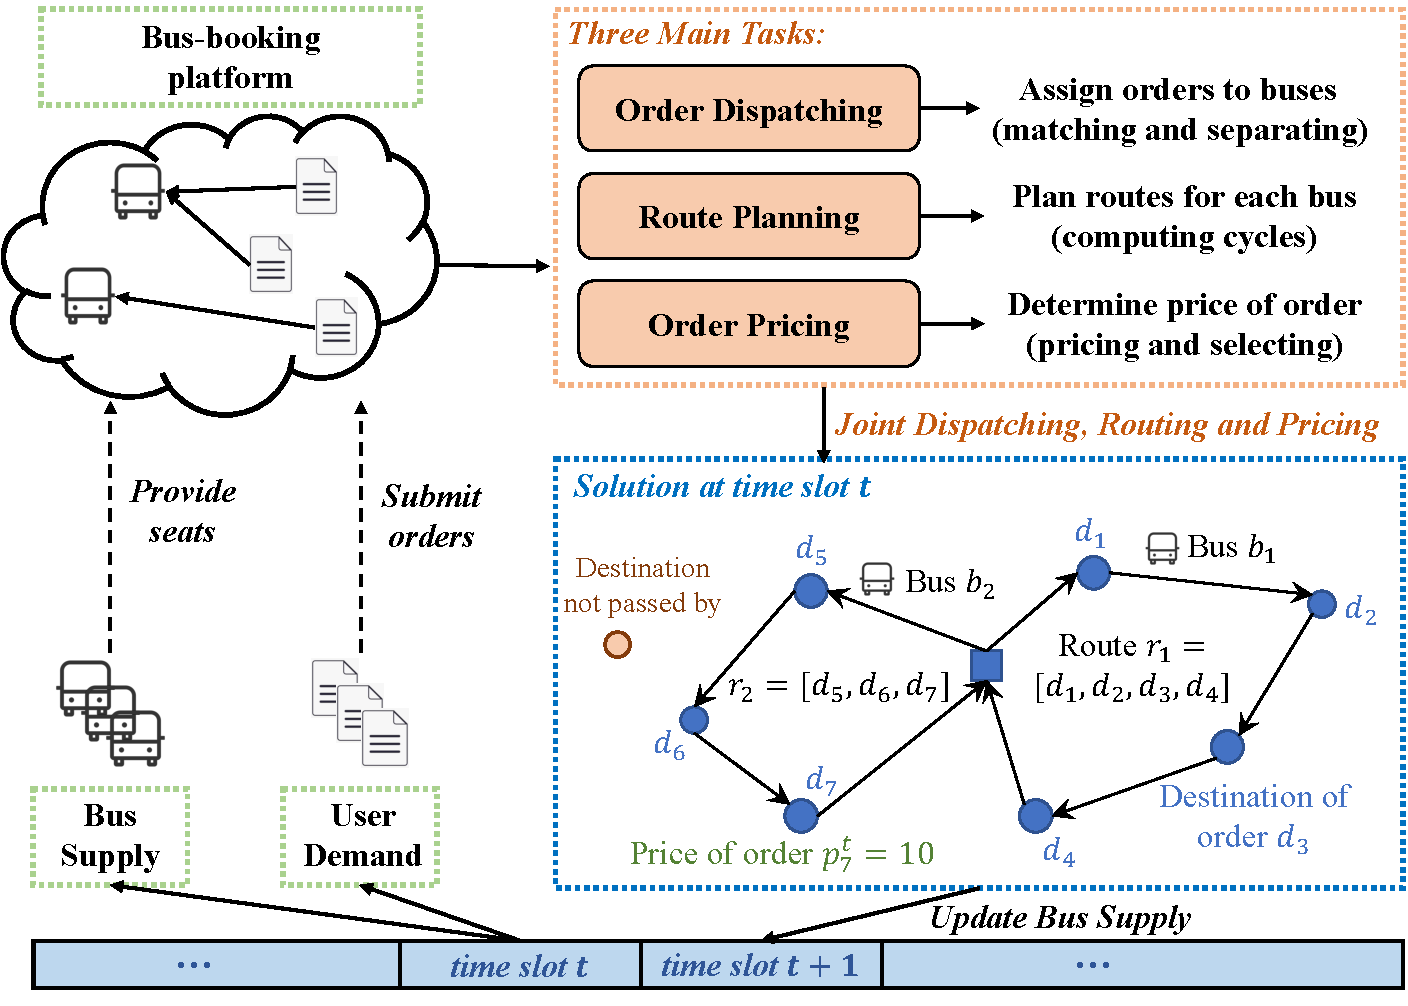
\includegraphics[width=0.85\linewidth]{fig/Overview.pdf}
        \caption{Flowchart of a bus-booking platform.}
        \label{fig:flow}
    \end{minipage}
\end{figure}

However, achieving an efficient and reliable bus-booking service is non-trivial. It requires the simultaneous optimization of three coupled decision-making tasks: \textit{Order Dispatching} (matching demands to vehicles), \textit{Route Planning} (sequencing destinations), and \textit{Trajectory Pricing} (determining fair and profitable fares). As illustrated in Figure~\ref{fig:flow}, \textcolor{blue}{these tasks are intrinsically interdependent. For instance, pricing strategies directly influence demand distribution, which dictates the feasibility of routes; conversely, route planning determines operational costs, which form the lower bound for pricing. Neglecting this coupling can lead to severe inefficiencies, such as accepting low-value orders that force excessive detours.}

% As shown in Figure~\ref{fig:flow}, the platform collects the bus supply and user demand information at each time slot, and utilizes some algorithms to match orders with buses, plan routes for different buses, and determine trajectory prices for different orders. The bus supply information at the next time slot is affected by the solution of the current time slot.

\color{blue}
To rigorously address these challenges, we formally define the \textbf{Joint order Dispatching, Route planning, and Trajectory Pricing (JDRP)} problem. We prove that JDRP is \textbf{NP-hard} via a reduction from the Traveling Salesman Problem (TSP). \textcolor{blue}{Beyond this inherent combinatorial complexity, the practical difficulty of the problem is further compounded by the specific assumptions regarding environmental dynamics:}
\begin{itemize}
    \item \textbf{The Stationary JDRP (S-JDRP):} This variant assumes stationary demand patterns. While easier to solve, this assumption often fails to reflect reality.
    \item \textbf{The Robust JDRP (R-JDRP):} Real-world platforms must cope with \textbf{dynamic uncertainty}, where demand intensity is non-stationary and governed by unknown distributions. This represents a more generalized and challenging form of the problem.
\end{itemize}

\color{black}

Existing commercial solutions, such as customized shuttles with uniform fares or chartered bus services, fail to solve the JDRP effectively due to their lack of granularity and flexibility~\cite{ref:JiangHCRide}. Similarly, traditional academic works often treat these coupled tasks in isolation (multi-stage approaches) or ignore the critical impact of environmental uncertainty~\cite{ref:dm, ref:DPEA, ref:PODP}. While recent research has progressed toward integrated solutions, such as jointly optimizing dispatching and routing~\cite{ref:odrp, ref:Lei2023}, few have established a unified framework that simultaneously optimizes all three tasks while explicitly ensuring robustness in non-stationary environments.

% the customized bus service and the chartered bus service provides flexible services. The customized bus service\footnote{\url{https://en.bcia.com.cn/jcbs.html#offSet}} means that the passenger can specify any destination within the city and the fare is uniformly $50$ CNY per person with a group of at least six persons. Simultaneously, the chartered bus service\footnote{\url{http://www.tx-trans.com/index.php/Index/GovOrder}} means that passengers can select proper chartered bus type, determine the time to use the bus and the destination of the journey. After the order is submitted, the platform will contact the passengers to confirm the service information. Although those specialized services address some traffic demand, the price of customized bus is unfair to passengers going to different destinations, and chartered buses cannot serve individual passenger~\cite{ref:JiangHCRide}.}

% In this paper, we propose an end-to-end method to solve the JDRP problem. We first design a novel framework named SACA, which synergizes Soft Actor-Critic (SAC) with attention mechanisms to fundamentally address the coupling of dispatching, routing, and pricing. While SACA effectively establishes the end-to-end optimization paradigm for stationary environments (S-JDRP), it treats spatial features as flat vectors and lacks mechanisms to handle volatility.

% SACA combines a SAC and an attention mechanism to maximize the long-term revenue of the JDRP problem. Specifically, SACA adopts a round-based model to cope with the online scenarios, where the entire processing procedure is cut into multiple equal-length time slots. At each time slot, } SACA determines the order price and the accepted order set according to the demand and supply relationship through the SAC framework, and then give the order dispatching and route planning solution with the attention mechanism, thus getting the new state of \textcolor{red}{the next time slot for SAC. With the iterative runs of the SAC and attention framework, we can get the dispatching, routing, and pricing solutions and gain high long-term revenue.}

% To address these real-world challenges, we further evolve SACA into a robust framework named ST-SACA. The core innovation of this extended version lies in the design of a Spatio-Temporal Adaptive Actor. This enhanced component explicitly integrates geographical coordinates with demand data via self-attention, enabling the agent to capture topological dependencies and learn robust strategies against dynamic uncertainty (R-JDRP). Consequently, ST-SACA inherits the joint optimization capability of SACA while equipping it with the necessary robustness for non-stationary environments.

% \textcolor{red}{However, the original SACA framework relies on a deterministic environment assumption, neglecting the dynamic uncertainty inherent in real-world operations, such as stochastic traffic conditions and fluctuating demand. Furthermore, it treats spatial inputs as flat features, ignoring the critical topological dependencies between stations. To address these challenges, we extend SACA to \textbf{ST-SACA}, a robust framework equipped with a \textbf{Spatio-Temporal Adaptive Actor}. Unlike the original flat architecture, our new actor explicitly integrates geographical coordinates with demand data using a self-attention mechanism. This allows the agent to capture \textbf{spatial topological dependencies} and learn robust pricing and routing strategies that adapt to environmental variations.}

\color{blue}
In this paper, we propose \textbf{ST-SACA}, a robust end-to-end framework designed to solve the JDRP problem. The framework is built upon a foundational Soft Actor-Critic (SAC) backbone synergized with attention mechanisms. This architecture fundamentally addresses the coupling of dispatching, routing, and pricing, establishing a unified optimization paradigm. However, standard architectures often treat spatial inputs as flat features, limiting their efficacy in non-stationary environments. To overcome this, ST-SACA distinguishes itself by incorporating a novel \textbf{Spatio-Temporal Adaptive Actor}. This enhanced component explicitly integrates geographical coordinates with demand data via self-attention, enabling the agent to capture topological dependencies and learn robust strategies against dynamic uncertainty. Consequently, ST-SACA not only inherits the joint optimization capability of the base model but also possesses the necessary robustness for real-world deployment.

Beyond the above innovations, we also ensure the framework's economic viability through a \textbf{realistic mechanism design}. We formulate the bilateral economic interaction between passengers and the platform by constructing distance-aware demand-supply functions and a composite reward scheme. These designs capture both passenger sensitivities and supply willingness, and balance conflicting operational objectives, ensuring ST-SACA's applicability in realistic settings.

\color{black}

We evaluate our methods using a real-world dataset. The experimental results demonstrate that our framework not only outperforms baselines in terms of the optimization objective but also exhibits superior robustness in uncertain scenarios.

\color{blue}
The main contributions are summarized as follows:
\begin{itemize}
    \item \textbf{Problem Formulation and Analysis:} We systematically formulate the JDRP problem for bus-booking platforms and rigorously prove its NP-hardness via a reduction from the TSP. Crucially, we \textbf{explicitly distinguish} between the \textbf{Stationary JDRP} and the \textbf{Robust JDRP}, establishing a formalized bridge between theoretical simplifications and real-world volatility.
    
    \item \textbf{End-to-End Robust Framework:} We propose \textbf{ST-SACA}, an end-to-end framework that jointly optimizes dispatching, routing, and pricing. ST-SACA incorporates a novel \textbf{Spatio-Temporal Adaptive Actor}, which explicitly integrates geographical topology with demand features via self-attention, enabling the agent to learn resilient strategies against environmental uncertainty.
    
    \item \textbf{Realistic Mechanism Design:} We formulate the \textbf{economic interaction} between passengers and the platform by constructing distance-aware demand and supply functions. These designs capture not only the heterogeneous price sensitivity of passengers but also the supply willingness of the platform. Furthermore, we construct a multi-objective composite reward function that balances profit, order response rate, and operational costs to guide the policy toward long-term optimality.
    
    \item \textbf{Extensive Real-World Validation:} We conduct comprehensive experiments using a real-world trajectory dataset. The results demonstrate that our model outperforms state-of-the-art baselines, and exhibits superior robustness and performance stability under non-stationary environments.
\end{itemize}



\section{Related Work} 
Given that order dispatching, route planning, and trajectory pricing are three pivotal components of the bus-booking ecosystem, we review the relevant literature from three perspectives: operational optimization in shared mobility, trajectory pricing mechanisms, and spatio-temporal modeling with robust learning.

\subsection{Order Dispatching and Route Planning in Shared Mobility} The fundamental operation of bus-booking platforms relies on efficiently matching orders to vehicles and planning optimal routes. Traditionally, order dispatching has been formulated as a bipartite matching problem or a constrained optimization problem. Early works largely employed exact algorithms or dynamic matching strategies with time windows to batch orders~\cite{ref:dm}. While effective for small-scale instances, these methods often struggle with the computational complexity of real-time massive requests. To address scalability, Multi-Agent Reinforcement Learning (MARL) has been extensively applied~\cite{ref:Yang2024KDD, ref:marl}, optimizing long-term platform efficiency~\cite{ref:Sun2022KDD}.

In the domain of route planning, heuristic algorithms and, more recently, machine learning techniques have gained prominence~\cite{tkde/ZhengCS23}. Neural Combinatorial Optimization (NCO) has emerged as a powerful alternative to traditional solvers. Pioneering works like Pointer Networks~\cite{ref_ptr} and Reinforcement Learning (RL) based approaches~\cite{ref_rl, ref:PanRoute} have demonstrated the capability to solve TSP and Vehicle Routing Problems (VRP) efficiently. Notably, the Transformer-based attention model proposed by Kool et al.~\cite{ref_att} significantly improved the quality and inference speed of routing solutions.

Despite these advancements, most existing studies treat dispatching and routing as sequential, independent tasks~\cite{ref:DPEA} or focus on specific sub-problems like demand-aware routing~\cite{ref:DemandAware}. Few frameworks achieve a truly end-to-end joint optimization of dispatching and routing while simultaneously considering the economic lever of pricing. Neglecting this coupling often leads to suboptimal solutions where accepted orders may incur excessive routing costs.

\subsection{Trajectory Pricing Mechanisms} Pricing serves as a crucial mechanism to balance supply and demand in transportation systems. Early strategies primarily relied on rule-based dynamic pricing (e.g., surge pricing) or statistical methods to maximize immediate revenue. For instance, Asghari et al.~\cite{ref:PODP} proposed an adaptive pricing scheme to guide supply towards high-demand regions. However, these myopic approaches often fail to optimize long-term horizons and are sensitive to short-term market noise.

To capture long-term dependencies, RL-based pricing strategies have been introduced~\cite{ref:Lei2023, ref:Ge2025}. A challenge is the continuous nature of price values. The standard Q-learning methods designed for discrete action spaces are not suitable for fine-grained pricing. While recent works attempted to handle continuous action spaces~\cite{ref:ROSDR}, they typically assume a homogeneous relationship between demand and price across different destinations.

In the context of bus-booking, pricing must be \textit{trajectory-aware}. Existing methods often overlook the spatial heterogeneity of operational costs. Orders with different destinations impose vastly different routing burdens on the bus. Our work addresses this by integrating a distance-aware demand-supply function within a continuous control RL framework.

\subsection{Spatio-Temporal Representation and Robust Learning} Effective decision-making in transportation requires capturing complex spatio-temporal dependencies. While early works relied on statistical models like ARIMA, deep learning approaches such as Graph Neural Networks (GNNs) and Attention mechanisms have become the state-of-the-art for modeling traffic flows~\cite{ref:STPivotal} and spatial correlations~\cite{ijcai/YuYZ18}. However, standard RL architectures used in dispatching often treat the system state as a flat feature vector, neglecting the underlying topological structure of the station network.

Furthermore, real-world operations are plagued by dynamic uncertainty. Standard RL assumes a stationary environment, leading to performance degradation when deployed in non-stationary real-world scenarios. Robust RL aims to learn policies resilient to environmental parameter variations~\cite{ref:RobustRoute, ref:RobustMARL} or out-of-distribution scenarios~\cite{ref:Yoon2024IJCAI}.

Although our preliminary work, SACA~\cite{ref:saca}, proposed a joint optimization framework, it relied on stationary environmental assumptions. There is a lack of unified frameworks that explicitly model the topological dependencies of station networks while ensuring robustness against non-stationary demand. Our proposed ST-SACA fills this void by introducing a Spatio-Temporal Adaptive Actor within a maximum entropy RL framework to cope with the non-stationary demand.

\section{Preliminaries and Problem Formulation}
\label{sec:problem}

In this section, we formally formulate the \textit{Joint order Dispatching, Route planning, and trajectory Pricing} (JDRP) problem. We first introduce the foundational entities and the general problem formulation. Subsequently, we discuss two variants of the JDRP problem: the \textit{Stationary JDRP} (S-JDRP)~\cite{ref:odrp} problem under stationary demand, and the \textit{Robust JDRP} (R-JDRP) problem under dynamic uncertainty. The key notations are summarized in Table~\ref{tab:not}.

%  Unlike traditional deterministic models, we incorporate dynamic uncertainty directly into the problem definition to reflect real-world operating conditions.

% We formulate the problem as a multi-stage decision-making process.

\begin{table}[!htbp]
\centering
\caption{\textcolor{blue}{Key Notations and Definitions}}
\footnotesize % 使用较小字号以适应单栏
\setlength{\tabcolsep}{0.3mm}
\label{tab:not}
\begin{center}
\begin{tabular}{c|c|l}
\toprule
\textbf{Category} & \textbf{Symbols} & \textbf{Description} \\
\midrule
\multirow{5}{*}{Sets \& Graph} 
 & $G$ & Station network (vertex set $V$, edge set $E$) \\
 & $loc_k$ & Coordinate $(x_k, y_k)$ of station $v_k \in V$ \\
 & $\mathcal{B}$ & Static fleet of all buses (Global set) \\
 & $\mathcal{B}^t$ & Set of available buses at time slot $t$ ($\mathcal{B}^t \subseteq \mathcal{B}$) \\
 & $\mathcal{O}^t$ & Batch of newly arrived orders at time slot $t$ \\
\midrule
\multirow{2}{*}{Uncertainty} 
 & $\mathcal{P}(\lambda^t)$ & Unknown non-stationary demand distribution \\
 & $\lambda^t$ & Time-varying demand intensity parameter \\
\midrule
\multirow{3}{*}{Order Entity} 
 & $o_j$ & Order index, $o_j \in \mathcal{O}^t$ \\
 & $d_j$ & Destination station of order $o_j$ \\
 & $c^o_j$ & Number of passengers for order $o_j$ \\
\midrule
\multirow{4}{*}{Bus Entity} 
 & $b_i$ & Bus index, $b_i \in \mathcal{B}$ \\
 & $r_i^t$ & Planned route sequence for bus $b_i$ at time $t$ \\
 & $L_i$ & Maximum passenger capacity of bus $b_i$ \\
 & $c^b_i$ & Current passenger load on bus $b_i$ \\
 & $v_i$ & Speed of bus $b_i$ \\
\midrule
\multirow{5}{*}{Calculation}
 & $T$ & Total operation time horizon \\
 & $\text{cost}_i$ & Operational cost for bus $b_i$ \\
 & $dis_i$ & Travel distance of the planned route $r_i^t$ \\
 & $\beta_d$ & Operational cost coefficient per unit distance \\
 & $p_j$ & Dynamic price offered to order $o_j$ \\
\midrule
\multirow{4}{*}{Decision \& Obj.} 
 & $x_{ij}^t$ & Binary decision for order-to-bus assignment \\
 & $\pi$ & Learned policy for platform \\
 & $R^t$ & Immediate profit at time slot $t$ \\
 & $\mathbb{E}[\sum R^t]$ & Total expected long-term profit over $T$ \\
\bottomrule
\end{tabular}
\end{center}
\end{table}

\subsection{Preliminaries}
\label{sec:pre}

For the bus-booking platform dedicated to the transportation hubs, buses are all departed from the same departure station, while orders can arrive at the platform at any time and their destinations can be anywhere within the city. To cope with the online scenarios of the bus-booking service, we adopt the round-based model referring to~\cite{ref_order_Zheng}. The foundational environment is modeled as follows.

\begin{definition}[Station Network]
The city station network is modeled as a graph $G=(V, E)$, where $V$ represents the set of stations (including the departure station $DS$ and all potential destinations), and $E$ represents the connectivity (road paths) between stations. Each station $v_k \in V$ is associated with a static coordinate $loc_k = (x_k, y_k)$. This spatial information defines the underlying topology of the network, which determines the travel distance between stations.
\end{definition}

\begin{definition}
(Time Horizon and Time Slot).
The operation time horizon $T$ of the platform is divided into equal-length time slots. In each slot $t$, the platform makes decisions based on the current state, which includes the batch of newly arrived orders $\mathcal{O}^t$ and the set of currently available buses $\mathcal{B}^t \subseteq \mathcal{B}$, where $\mathcal{B}$ represents the entire static fleet.
\end{definition}

\begin{definition}
(Demand).
In real-world scenarios, passenger demand is stochastic and fluctuates over time. We model the underlying demand potential at station $k$ during time slot $t$ as a variable governed by a time-dependent probability distribution $\mathcal{P}(\lambda^t_k)$, where $\lambda^t_k$ represents the varying demand intensity. Crucially, this distribution is \textbf{unknown} to the platform.
\end{definition}

\begin{definition}
(Order).
At the beginning of each time slot $t$, a batch of orders $\mathcal{O}^t$ arrives at the platform. The platform observes this batch to make decisions. Each specific order $o_j \in \mathcal{O}^t$ is defined as a tuple $\langle d_j, c_j^o \rangle$, where $d_j \in V$ is the destination station and $c^o_j$ is the number of passengers.
\end{definition}

\color{black}
\begin{definition}
(Bus).
A bus $b_i \in \mathcal{B}^t$ is represented by a tuple $\langle r_i, L_i, c^b_i, v_i \rangle$, where $r_i$ is the route sequence starting and ending at $DS$, $L_i$ is the capacity limit, $c^b_i$ is the current load, and $v_i$ is the average bus speed.
\end{definition}

\subsection{Problem Formulation}
\label{sec:formulate}

The objective of the JDRP problem is to maximize the platform's long-term profit under dynamic uncertainty. Four constraints are required to ensure solution feasibility.

\begin{itemize}
    \item \textbf{Uniqueness constraint:} Each accepted order $o_j$ is assigned to exactly one bus.
    \item \textbf{Capacity constraint:} The number of passengers on bus $b_i$ cannot exceed its capacity $L_i$.
    \item \textbf{Precedence constraint:} If an order $o_j$ is assigned to a bus $b_i$, its destination $d_j$ must be visited by the bus. 
    \item \textbf{Loop constraint:} All buses must start and end at $DS$.
\end{itemize}

\color{blue}

Let $x_{ij}^t \in \{0, 1\}$ be the binary decision variable and $p_j$ be the dynamic price offered for order $o_j$, where $x_{ij}^t=1$ implies that order $o_j$ is assigned to bus $b_i \in \mathcal{B}^t$. We can formulate the profit in time slot $t$ and the JDRP problem as follows.

\begin{definition}
    (Platform Profit). The platform's profit in time slot $t$ for a given order set $\mathcal{O}^t$ and bus set $\mathcal{B}^t$ is
    \begin{equation}
        R^t = \sum_{o_j \in \mathcal{O}^t} \left( p_j \cdot \sum_{b_i \in \mathcal{B}^t} x_{ij}^t \right) - \sum_{b_i \in \mathcal{B}^t} \text{cost}_i,
    \end{equation}
    where $\text{cost}_i = \beta_d \cdot dis_i$ is the operational cost for bus $b_i$, with $dis_i$ being the travel distance for bus $b_i$, and $\beta_d$ is the cost per unit distance.
\end{definition}

\begin{definition}(JDRP Problem).
Given the station network $G$ and the bus fleet $\mathcal{B}$, consider an environment where the passenger demand is governed by an unknown stochastic process. \textbf{Joint order Dispatching, Route planning, and trajectory Pricing (JDRP)} problem aims to learn a policy $\pi$ that generates the decision tuple $\langle \mathbf{Price}^t, \mathbf{X}^t, \mathbf{Route}^t \rangle$ for $\mathcal{O}^t$, $\mathcal{B}^t$ to maximize the \textbf{expected} long-term profit over the horizon $T$, subject to the above constraints. The formulation is as follows:
\begin{eqnarray}
    \max_{\pi} & \sum_{t=1}^T \mathbb{E}_{\mathcal{O}^t \sim \mathcal{P}(\lambda^t)}\left[R^t\right] \\
    \text{ s.t. } & \sum_{b_i \in \mathcal{B}^t} x_{ij}^t \leq 1, \quad \forall o_j \in \mathcal{O}^t \label{eq:unique} \\
    & \sum_{o_j \in \mathcal{O}^t} x_{ij}^t \cdot c^o_j \leq L_i, \quad \forall b_i \in \mathcal{B}^t \label{eq:capacity} \\
    & d_j \in r_i, \quad \forall x_{ij}^t = 1 \label{eq:prec} \\
    & r_i[0] = r_i[-1] = DS, \quad \forall b_i \in \mathcal{B}^t \label{eq:loop} \\
    & \forall t \in \{1, \dots, T\} \nonumber
\end{eqnarray}
\end{definition}

% 建议插入到 3.2 Problem Formulation 的末尾
\subsection{Problem Variants under Stationarity Assumptions}
\label{sec:stationarity_def}

The complexity of the JDRP problem relies heavily on the temporal properties of passenger demand. We formulate two problem variants based on the \textbf{stationarity assumption} of the demand distribution.

\textbf{1) The Stationary JDRP (S-JDRP):}
This variant operates under the assumption that the demand distribution is \textbf{stationary} over time. In this setting, demand patterns are stable or strictly cyclic. This formulation aligns with the assumptions made in our preliminary work~\cite{ref:odrp} and most traditional multi-stage approaches.

\textbf{2) The Robust JDRP under Non-Stationarity (R-JDRP):}
This variant relaxes the stationarity assumption to model realistic urban dynamics. Here, the demand intensity is governed by a \textbf{non-stationary} stochastic process with unknown distributional shifts. This represents a generalized and more challenging form of the problem, requiring algorithms with strong adaptability and robustness.

\subsection{Case Study and NP-Hardness Analysis}

\begin{figure}[htbp]
    \centering
    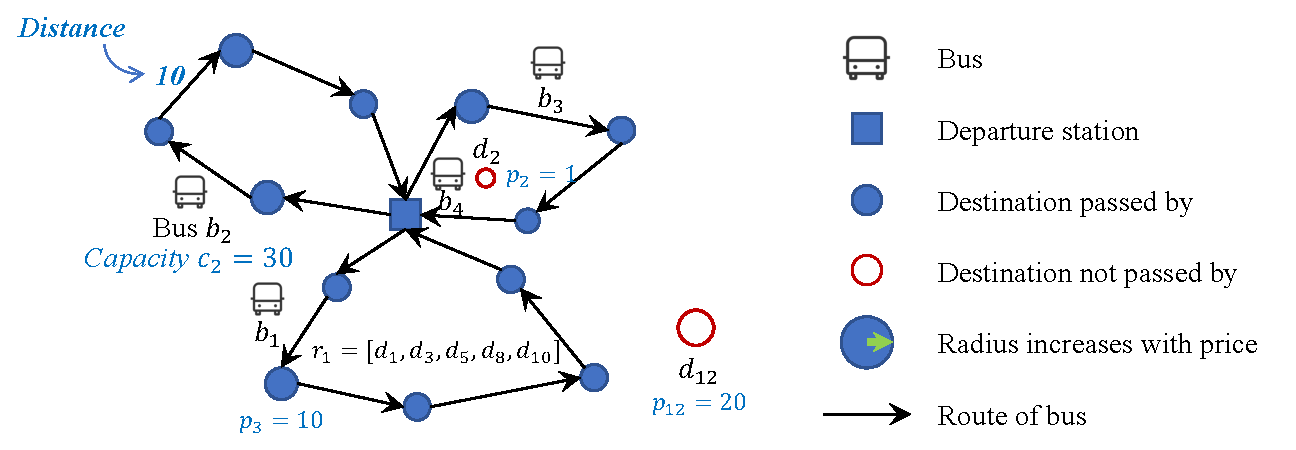
\includegraphics[width=\linewidth]{fig/toyexample.pdf}
    \caption{\textcolor{blue}{A toy example.}}
    \label{fig:toy}
\end{figure}

The JDRP problem involves joint decision-making across three coupled tasks. The platform must simultaneously balance pricing (to filter demand), dispatching (to match capacity), and routing (to minimize cost). A toy example of a single time slot for the JDRP problem is shown in Figure~\ref{fig:toy}, where the solid point represents the departure station $DS$, each point represents the destination of the passenger, and edges represent planned routes. In the toy example, four buses depart from the same departure station $DS$, while some orders with different destinations are submitted to the platform. Under constraints mentioned above, the platform decides which orders to accept, determines their prices, and plans routes for buses to maximize the profit, while may reserve some buses for use in the next time slot, such as $b_4$. $d_2$ and $d_{12}$ denoted by red hollow points are rejected. Specifically, though $d_2$ is close to $DS$ which implying the cost for platform to passing by $d_2$ is low, a low price of orders to $d_2$ results in rejection. $d_{12}$ is not passed by because $d_{12}$ is far from $DS$. Besides, the route of $b_1$ consists of destinations of the orders assigned to the bus, i.e., $r_1 = [d_1, d_3, d_5, d_8, d_{10}]$. %Toy example

We prove the JDRP problem is NP-hard via a reduction from the Traveling Salesman Problem (TSP).

\begin{proof}
Consider a simplified instance with a single time slot, one bus with infinite capacity, and deterministic traffic. If we fix the price such that all orders must be accepted to maximize the profit, the problem reduces to finding the shortest path visiting all destinations and returning to the depot, which is exactly the TSP. Since TSP is NP-hard, the more general JDRP is also NP-hard.
\end{proof}

\section{The ST-SACA Framework}
\label{sec:framework}

The proposed \textbf{ST-SACA} framework is an end-to-end solution designed to address the JDRP problem under dynamic uncertainty. 
As illustrated in Figure~\ref{fig:framework}, the framework operates in a hierarchical manner: 
(1) The \textbf{Demand-Supply Interaction} module models how market demand responds to pricing strategies; 
(2) The \textbf{Robust Trajectory Pricing and Dispatching} module, powered by a Spatio-Temporal Adaptive Actor-Critic agent, determines the optimal pricing and seat allocation to maximize long-term profit; 
(3) The \textbf{Attention-Based Routing} module utilizes an attention-based network to execute efficient route planning based on the pricing and dispatching decisions.

\begin{figure}[htbp]
\centering
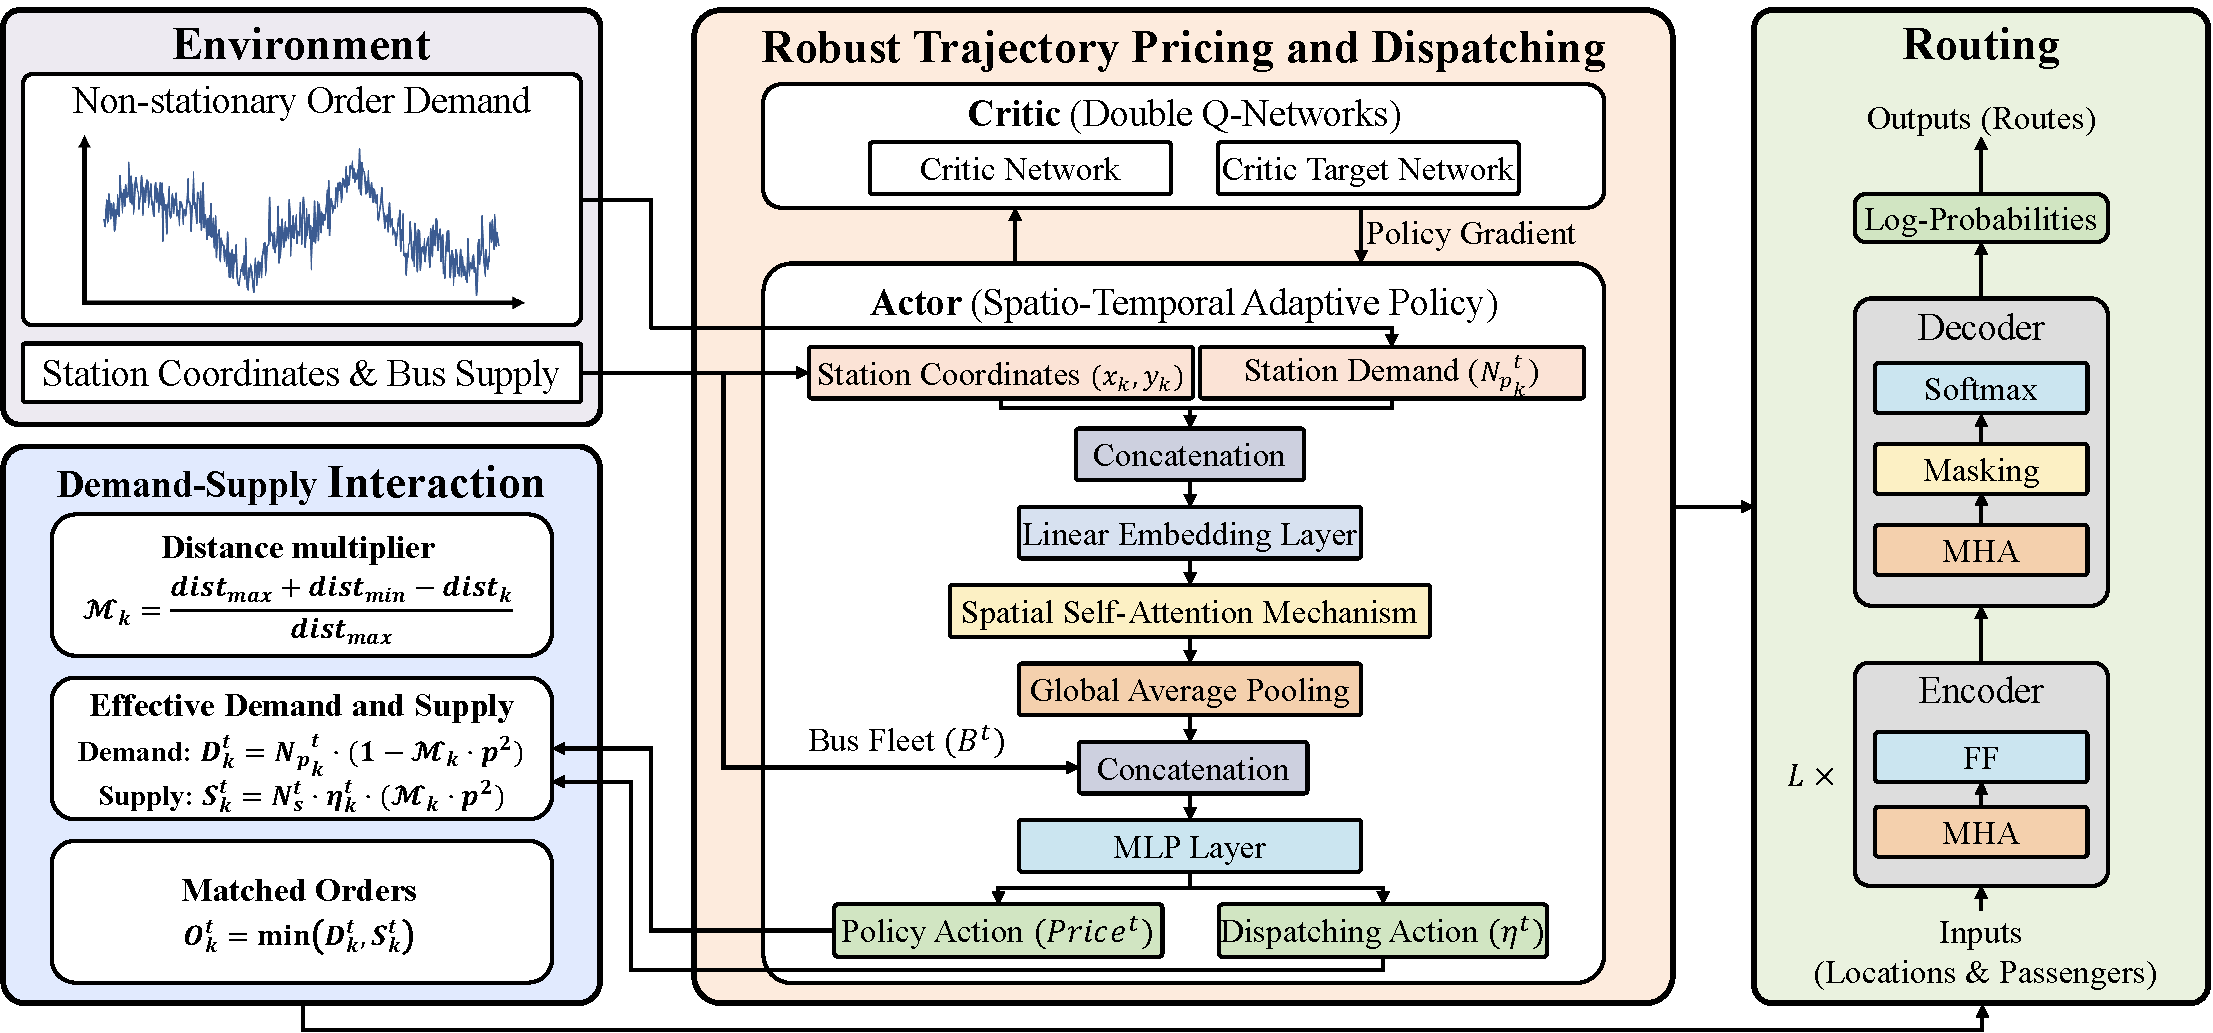
\includegraphics[width=\columnwidth]{fig/Framework-journal.pdf}
\caption{\textcolor{blue}{Overview of the ST-SACA method.}}\label{fig:framework}
\end{figure}

\color{black}
\subsection{Demand-Supply Interaction Modeling}
\label{sec:candidate}
To simulate the dynamic market environment, we model the interaction between platform pricing and passenger demand.
At each time slot $t$, let ${N_p}^t_k$ denote the number of potential passengers intending to go to destination $k$. This value is a realization derived from the stochastic demand process $\mathcal{O}^t \sim \mathcal{P}(\lambda^t)$ defined in Section~\ref{sec:pre}.

We define a demand-price sensitivity function $F_{pk}(p)$ to quantify the acceptance probability of passengers at destination $k$ under price $p$. 
Simultaneously, the platform controls the supply distribution via an allocation function $F_{sk}(p)$.
The effective demand $D^t_k$ and supply capacity $S^t_k$ for destination $k$ are formulated as:
\begin{equation}
    D^t_k(p^t_k) = {N_p}^t_k \cdot F_{pk}(p^t_k),
\end{equation}
\begin{equation}
    S^t_k(p^t_k) = N_{s}^t \cdot \eta^t_k \cdot F_{sk}(p^t_k),
\end{equation}
where $N_{s}^t$ is the total number of available seats in the current bus set $\mathcal{B}^t$, and $\eta^t_k$ is the fraction of seats allocated to destination $k$ with $\sum_k \eta^t_k = 1$.

Considering the spatial heterogeneity, we model the divergent preferences of passengers and the platform regarding travel distance. 
From the demand side, passengers traveling to farther destinations typically exhibit \textbf{lower price sensitivity} due to the lack of convenient alternatives. 
Conversely, from the supply side, the platform prefers allocating resources to closer destinations to \textbf{minimize operational costs} and avoid excessive detours. 
To capture this trade-off, we incorporate a distance-based multiplier $\mathcal{M}_k$ into both functions:
\begin{equation}
    F_{pk}(p) = 1 - \mathcal{M}_k \cdot p^2, \quad F_{sk}(p) = \mathcal{M}_k \cdot p^2,
\end{equation}
where $\mathcal{M}_k = \frac{dist_{max} + dist_{min} - dist_{k}}{dist_{max}}$ serves as the distance factor. 
Here, $dist_{k}$ denotes the distance between station $k$ and the departure station $DS$ while $dist_{max}$ and $dist_{min}$ are the maximum and minimum distances in the network, respectively. 
Specifically, a larger $dist_k$ results in a smaller $\mathcal{M}_k$, which simultaneously models the high price tolerance of long-distance passengers and the platform's reluctance to serve high-cost distant orders at low prices.

Consequently, the number of successfully dispatched orders $O^t_k$ and the immediate profit $R^t$ are calculated as:
\begin{equation}
    O^t_k = \min(D^t_k, S^t_k), \quad R^{t} = \sum_k p^t_k O^t_k - \sum_{b_i \in \mathcal{B}^t} \text{cost}_i.
\end{equation}

\subsection{Robust Trajectory Pricing and Dispatching}
\label{sec:sac}

This module serves as the decision-making core of the ST-SACA framework. To address the continuous nature of pricing control and the stochasticity of passenger demand, we model the problem as a Markov Decision Process (MDP) and employ a customized Soft Actor-Critic (SAC) algorithm. The continuous action spaces and maximum entropy objective of SAC is particularly suitable for this task, as it encourages exploration, preventing the policy from collapsing into suboptimal deterministic behaviors in uncertain environments.

\subsubsection{MDP Formulation}
We define the tuple $\langle \mathcal{S}, \mathcal{A}, \mathcal{R}, \mathcal{T} \rangle$ for the pricing and dispatching decision as follows:

\textbf{State ($\mathcal{S}$):} 
The state $s^t$ encapsulates both the dynamic market demand and the supply status of the platform at time slot $t$. Formally, $s^t = \langle \mathbf{N}_p^t, \mathbf{B}^t \rangle$. 
Here, $\mathbf{N}_p^t = [{N_p}^t_k]_{k \in |V|}$ represents the potential demand vector across all stations. 
$\mathbf{B}^t=\{\tau_i^t\}_{b_i \in \mathcal{B}}$ denotes the fleet status, where $\tau_i^t$ indicates the remaining time required for bus $b_i$ to return to $DS$. If $\tau_i^t = 0$, the bus is idle and available for dispatch.

\textbf{Action ($\mathcal{A}$):} 
The action vector $a^t$ comprises two coupled decisions: trajectory pricing and seat allocation. We define $a^t = \langle \mathbf{Price}^t, \boldsymbol{\eta}^t \rangle$, where $\mathbf{Price}^t = [p^t_k]_{k \in |V|} \in [0, 1]^{|V|}$ is the normalized price vector offered to passengers at each destination. $\boldsymbol{\eta}^t = [\eta^t_k]_{k \in |V|}$ represents the distribution of available seats allocated to different destinations.

\textbf{Reward ($\mathcal{R}$):} 
To ensure the sustainability of the platform, the reward function must balance immediate profitability with service quality. We define the reward $Reward^t$ as a weighted sum of the profit $R^t$ and the Order Response Rate ($ORR^t$):
\begin{equation}
    Reward^t = R^t + \lambda_{orr} \cdot ORR^t,
\end{equation}
where $R^t$ is the revenue minus operational costs (as defined in Eq. (5)), and $ORR^t = (\sum_k O^t_k) / (\sum_k D^t_k)$ quantifies the platform's ability to satisfy demand. The coefficient $\lambda_{orr}$ balances the profit maximization and service responsiveness.

\textbf{Transition ($\mathcal{T}$):} 
The state transition is governed by the dynamics of order fulfillment and fleet circulation. The available capacity for the subsequent time slot, $N_{s}^{t+1}$, is updated based on the number of newly dispatched buses and returning buses:
\begin{equation}
    N_{s}^{t+1} = N_{s}^t - \sum_{b_i \in \mathcal{B}^t_{disp}} L_i + \sum_{b_j \in \mathcal{B}} \mathbb{I}(\tau^t_j \le \Delta t) \cdot L_j,
\end{equation}
where $\mathcal{B}^t_{disp}$ is the set of buses dispatched at $t$, $\mathbb{I}(\cdot)$ is the indicator function, and $\Delta t$ is the duration of a time slot.

\color{blue}
\subsubsection{Spatio-Temporal Adaptive Actor}
\label{sec:actor}
Standard reinforcement learning approaches often treat the spatial state $\mathbf{N}_p^t$ as a flat feature vector, neglecting the underlying topological dependencies between stations. However, in urban transportation, demand fluctuations and destination locations are often spatially correlated. To enhance robustness, we design a \textit{Spatio-Temporal Adaptive Actor} that explicitly captures the topological dependencies.

\textbf{Coordinate-Aware Embedding:} 
First, we fuse the dynamic demand with static geographical information. For each station $k$, we construct a raw feature vector $v_k = [{N_p}^t_k, x_k, y_k]$, where $(x_k, y_k)$ are the normalized coordinates. This vector is projected into a high-dimensional embedding space via a learnable transformation:
\begin{equation}
    \mathbf{e}_k = \text{ReLU}(\mathbf{W}_e \cdot v_k + \mathbf{b}_e).
\end{equation}

\textbf{Spatial Self-Attention Mechanism:} 
We employ a multi-head self-attention mechanism to model the interactions between stations and dynamically weigh the influence of different stations based on current market conditions. The attention coefficient $\alpha_{i,j}$ describes the dependency of station $i$ on $j$:
\begin{equation}
    \alpha_{i,j} = \text{softmax}_j\left(\frac{(\mathbf{e}_i\mathbf{W}_Q)(\mathbf{e}_j\mathbf{W}_K)^T}{\sqrt{d_k}}\right),
\end{equation}
where $\mathbf{W}_Q$ and $\mathbf{W}_K$ are query and key projection matrices, and $d_k$ is the dimension of the keys. The spatially context-aware feature representation $\mathbf{h}_i$ is then updated by aggregating information from the entire network:
\begin{equation}
    \mathbf{h}_i = \mathbf{e}_i + \sum_{j \in |V|} \alpha_{i,j} (\mathbf{e}_j\mathbf{W}_V).
\end{equation}

The mechanism can identify "hotspot" regions and propagate demand information across the topology.

\textbf{Global Policy Generation:} 
Finally, to generate a unified policy for the entire platform, we apply global average pooling to the station-specific features to obtain a permutation-invariant graph representation $\mathbf{s}_{global}$:
\begin{equation}
    \mathbf{s}_{global} = \frac{1}{|V|} \sum_{k \in |V|} \mathbf{h}_k.
\end{equation}

The global state $\mathbf{s}_{global}$ is concatenated with the bus fleet status encoding and fed into the policy network to output the action $a^t$. This architecture ensures that the pricing strategy is adaptive not only to temporal demand shifts but also to the spatial distribution of orders.

\color{black}
\subsection{Attention-Based Routing}
\label{sec:routing}
Once the pricing strategy $a^t$ determines the set of accepted orders, the system must solve the routing problem to minimize operational costs. 
Exact algorithms are computationally prohibitive due to the NP-hard nature of the routing problem. Similarly, conventional meta-heuristics (e.g., Genetic Algorithms or Tabu Search) require extensive iterative search processes from scratch for each new batch, leading to unacceptable latency for real-time platforms. 
To address this, we employ a machine learning approach based on the Transformer architecture~\cite{ref_att}. 
Compared to traditional methods, this learning-based approach offers two distinct advantages: 
(1) \textbf{Real-time Inference}: Once trained, the model acts as a fast heuristic that generates high-quality solutions in milliseconds, satisfying the instant response requirement of bus-booking platforms.
(2) \textbf{Sequence Agnostic}: The underlying attention mechanism inherently handles input sequences of varying lengths, allowing the model to adapt seamlessly to fluctuating routing requirements at different time slots.

\textbf{Encoder (Context Aggregation):} 
The encoder maps the DS and destinations of the accepted orders into a sequence of context-aware embeddings. 
For a station $k$ with coordinate $loc_k$, the initial embedding is $h_k^{(0)} = \mathbf{W}_{emb} loc_k + \mathbf{b}_{emb}$. 
Crucially, we utilize $L$ layers of Multi-Head Attention (MHA) followed by Batch Normalization (BN) and Feed-Forward (FF) layers to capture the global topological dependencies between stations and update the embeddings.
\begin{gather}
    \hat{h}_k = \text{BN}(h_k^{(l-1)} + \text{MHA}_k(h_1^{(l-1)}, \dots, h_N^{(l-1)})), \\
    h_k^{(l)} = \text{BN}(\hat{h}_k + \text{FF}(\hat{h}_k)).
\end{gather}

\textbf{Decoder (Attention-Based Pointer):} 
The decoder constructs the route sequentially using an attention-based pointer mechanism. 
At each step $j$, the decoder computes an attention distribution over all encoder embeddings to probabilistically select the next station. 
The attention score $u_{k}^{i}$, which reflects the compatibility between the current decoding context and candidate station $k$, is calculated as:
\begin{gather}
    u_{k}^{j} = C \cdot \tanh(\mathbf{W}_{q} h_{decoder}^j + \mathbf{W}_{k} h_{k}^{(L)}), \label{eq:att} \\
    p(k | r_{1:j-1}) = \text{softmax}(u^j), \label{eq:pro}
\end{gather}
where $r_{1:j-1}$ denotes the partial route visited so far. Here, masking techniques are applied to ensure constraints (loop to $DS$) are satisfied. The decoder outputs the proper route $r_i$, which determines the cost term in the SAC reward function.

\color{blue}
\begin{algorithm}[tb]
\caption{Attention-Based Route Generation}
\label{alg:routing}
\begin{algorithmic}[1]
\REQUIRE Accepted Order Set $\hat{\mathcal{O}}^t$, Bus Set $\mathcal{B}^t$, Trained Attention Model $\mathcal{M}$
\ENSURE Bus routes $\mathbf{Route}^t = \{r_1, \dots, r_{|\mathcal{B}^t|}\}$
\STATE \textbf{Encoder:} Compute context-aware embeddings $H = \{h_j\}$ for all $d_j \in \hat{\mathcal{O}}^t \cup \{DS\}$ using model $\mathcal{M}$
\FOR{each bus $b_i \in \mathcal{B}^t$}
    \STATE Initialize route $r_i \leftarrow [DS]$
    \STATE Initialize decoder state $h_{decoder} \leftarrow h_{DS}$ \COMMENT{Start with Depot embedding}
    \STATE Mark $DS$ as visited
    \WHILE{bus $b_i$ has not returned to $DS$}
        \STATE \textbf{Masking:} Identify invalid nodes $\mathcal{V}_{invalid}$ (visited)
        \STATE Set attention scores: $u_k \leftarrow -\infty, \forall v_k \in \mathcal{V}_{invalid}$
        \STATE \textbf{Attention:} Compute probability via Eq. (13) and (14)
        \STATE \textbf{Selection:} Select next node $v_{next} = \arg\max P$
        
        \IF{$v_{next}$ is $DS$}
            \STATE Break inner loop
        \ELSE
            \STATE Append $v_{next}$ to $r_i$ and mark $v_{next}$ as visited
            \STATE Update decoder state: $h_{decoder} \leftarrow h_{v_{next}}$
        \ENDIF
    \ENDWHILE
    \STATE Append $DS$ to $r_i$
\ENDFOR
\RETURN $\mathbf{Route}^t$
\end{algorithmic}
\end{algorithm}

\subsection{Summary of Algorithm Workflow}
\label{sec:workflow}

Integrating the Spatio-Temporal Adaptive Actor and the Attention-based Routing module, we present the overall training and execution workflow of ST-SACA.

\textbf{Training Phase:} Algorithm~\ref{alg:training} outlines the training procedure. The framework alternates between interacting with the environment to collect experiences and updating the network parameters. The reward calculation in line~\ref{line:reward} relies on the route distance computed by the routing module.

\begin{algorithm}[tb]
\caption{ST-SACA Policy Training} % 优化后的名称，强调策略学习
\label{alg:training}
\begin{algorithmic}[1]
\REQUIRE Pre-trained Routing Model $\mathcal{M}$, Environment Params
\ENSURE Optimized Policy $\pi_\phi$, Critic Networks $Q_{\theta_1}, Q_{\theta_2}$
\STATE \textbf{Initialization:} 
\STATE \quad Init Actor $\pi_\phi$, Critics $Q_{\theta_1}, Q_{\theta_2}$, Target Critics $Q_{\bar{\theta}_1}, Q_{\bar{\theta}_2}$
\STATE \quad Init Replay Buffer $\mathcal{D}$ with capacity $C$
\FOR{episode $ep = 1$ to $MaxEp$}
    \STATE Reset environment, observe initial state $s^1 = \langle \mathbf{N}_p^1, \mathcal{B}^1 \rangle$
    \FOR{time slot $t = 1$ to $T$}
        \STATE \textbf{I. Spatio-Temporal Decision}
        \STATE Generate embeddings $\mathbf{e}_k$ and global state $\mathbf{s}_{global}$
        \STATE Sample action $a^t \sim \pi_\phi(\cdot|s^t)$

        \STATE \textbf{II. Environment Interaction}
        \STATE Generate routes $\mathbf{Route}^t$ via \textbf{Alg.~\ref{alg:routing}} using Model $\mathcal{M}$
        \STATE Calculate Reward and observe next state $s^{t+1}$ \label{line:reward}
        \STATE Store transition tuple $(s^t, a^t, Reward^t, s^{t+1})$ into $\mathcal{D}$
        
        \STATE \textbf{III. SAC Parameter Update}
        \STATE Sample minibatch from $\mathcal{D}$
        \STATE Update Critics $\theta_i$ by minimizing Bellman error
        \STATE Update Actor $\phi$ by maximizing entropy objective
        \STATE Soft update target networks: $\bar{\theta}_i \leftarrow \tau\theta_i + (1-\tau)\bar{\theta}_i$
    \ENDFOR
\ENDFOR
\end{algorithmic}
\end{algorithm}

\textbf{Online Execution:} Once trained, the model is deployed for real-time decision-making. As shown in Algorithm~\ref{alg:online_execution}, the inference is efficient. The pricing and dispatching policy and routing model work sequentially within each time slot to handle the dynamic order batch.

\begin{algorithm}[tb]
\caption{Online Execution Procedure (Per Time Slot)}
\label{alg:online_execution}
\begin{algorithmic}[1]
\REQUIRE Current Time Slot $t$, Real-Time Demand $\mathbf{N}_p^t$, Available Bus Set $\mathbf{B}^t$, Trained Models $\pi_\phi, \mathcal{M}$
\ENSURE Pricing Vector $\mathbf{Price}^t$, Dispatching Solution $\mathbf{X}^t$, Bus Routes $\mathbf{Route}^t$
\STATE \textbf{Phase I: State Construction}
\STATE Generate spatial-aware embeddings for current demand
\STATE Construct state vector: $s^t \leftarrow \langle \mathbf{N}_p^t, \mathbf{B}^t \rangle$

\STATE \textbf{Phase II: Robust Pricing and Dispatching}
\STATE Generate action $a^t = \langle \mathbf{Price}^t, \boldsymbol{\eta}^t \rangle \leftarrow \pi_\phi(s^t)$ 
\STATE Derive accepted order set $\hat{\mathcal{O}}^t$

\STATE \textbf{Phase III: Routing Generation}
\STATE $\mathbf{Route}^t \leftarrow \text{RouteGeneration}(\hat{\mathcal{O}}^t, \mathbf{B}^t, \mathcal{M})$

\STATE \textbf{Phase IV: System Execution}
\STATE Publish prices $\mathbf{Price}^t$ to user platform
\STATE Dispatching orders and buses according to $\mathbf{X}^t$ and $\mathbf{Route}^t$
\STATE Update bus fleet status based on route durations
\RETURN $\mathbf{Price}^t, \mathbf{Route}^t$
\end{algorithmic}
\end{algorithm}

\subsection{Theoretical Analysis}
\label{sec:theory}

In this section, we provide a rigorous analysis of the computational complexity and the theoretical properties concerning the convergence and robustness of the proposed ST-SACA.

\subsubsection{Computational Complexity Analysis}
The real-time inference process in each time slot is composed of two sequential phases: the pricing and dispatching phase executed by the Spatio-Temporal Adaptive Policy Actor and the routing phase executed by the Attention-based Routing module. Let $d$ denote the feature embedding dimension (i.e., the size of vectors $\mathbf{e}_k$ in Eq. (8) and $h_k$ in Eq. (11)). Note that the key dimension $d_k$ used in Eq. (9) is typically proportional to $d$ (e.g., $d_k = d/H$ in multi-head attention), so the asymptotic complexity is governed by $d$.

\textbf{Pricing and Dispatching Phase Complexity:} 
The core computational overhead of the pricing and dispatching actor stems from the self-attention mechanism. For an input sequence of length $|V|$, the time complexity of calculating the attention scores is $O(|V|^2 \cdot d)$, while the subsequent feed-forward layers require $O(|V| \cdot d^2)$. Consequently, the total complexity for the pricing and dispatching phase is $O(|V|^2 \cdot d + |V| \cdot d^2)$. Given that the number of stations $|V|$ in a typical bus-booking scenario is relatively small (e.g., $|V| \approx 30$ in our experiments), this quadratic dependency remains computationally lightweight.

\textbf{Routing Phase Complexity:} 
Let $M$ be the number of destinations of accepted orders, where $M \leq |V|$. The routing module employs an encoder-decoder architecture. The encoder processes the station embeddings with a self-attention complexity of $O(M^2 \cdot d)$. The decoder generates the route auto-regressively. Each decoding step performs an attention operation over the $M$ encoder outputs, incurring $O(M \cdot d)$ cost. Thus, the total decoding complexity is $O(M^2 \cdot d)$.

\textbf{Overall Complexity:} 
The aggregate inference complexity per time slot is $O((|V|^2 + M^2) \cdot d)$. This polynomial complexity ensures that ST-SACA can generate solutions within milliseconds, satisfying the real-time requirements of online bus-booking platforms.

\subsubsection{Convergence and Robustness Properties}
The ST-SACA framework is theoretically grounded in the maximum entropy reinforcement learning paradigm, which offers distinct advantages in terms of convergence stability and robustness against environmental uncertainty.

\textbf{Convergence Guarantee:} 
ST-SACA optimizes the maximum entropy objective:
\begin{equation}
    J(\pi) = \sum_{t=1}^T \mathbb{E}_{(s^t, a^t) \sim \rho_\pi} [r(s^t, a^t) + \alpha \mathcal{H}(\pi(\cdot|s^t))].
\end{equation}
Based on the Soft Policy Iteration theorem~\cite{icml/HaarnojaZAL18}, the tabular version of Soft Actor-Critic guarantees monotonic improvement in the Q-value function, i.e., $Q_{new}(s,a) \ge Q_{old}(s,a)$ for all $(s,a)$, leading to the optimal maximum entropy policy. In our continuous state-space implementation using neural function approximators, the inclusion of the entropy term $\alpha \mathcal{H}(\pi(\cdot|s_t))$ effectively convexifies the optimization landscape locally, preventing the policy from premature convergence to sub-optimal deterministic behaviors—a common pitfall in standard actor-critic methods.

\textbf{Theoretical Robustness:} 
The robustness of ST-SACA against uncertainty $\lambda^t$ is derived from two key components:
\begin{itemize}
    \item \textbf{Lipschitz Continuity of State Representation:} The Spatio-Temporal Adaptive Actor utilizes coordinate-aware embeddings combined with self-attention. This architecture ensures that the learned state representation $\mathbf{s}_{global}$ is Lipschitz continuous with respect to spatial input perturbations. Specifically, small variations in local demand $N_p^t$ result in bounded changes in the aggregated state $\mathbf{s}_{global}$. This smoothness stabilizes the value function approximation $Q_\theta(s, a)$, reducing the variance of gradient estimates under high uncertainty.
    \item \textbf{Entropy-Regularized Resilience:} Unlike deterministic policies that overfit to specific trajectory instances, the maximum entropy objective encourages the agent to learn a stochastic policy that captures multiple high-reward modes. This acts as a robust regularizer, enabling the agent to maintain high performance even when the test environment (e.g., demand distribution $\mathcal{P}(\lambda^t)$) deviates slightly from the training distribution.
\end{itemize}

Empirically, these properties translate to the superior stability and faster convergence observed in Figure~\ref{fig:exper_curve}.

\section{Experiments}
\label{sec:experiments}

In this section, we evaluate the performance of ST-SACA on real-world datasets. 

% aiming to answer the following questions:
% \begin{itemize}
%     \item \textbf{RQ1 (Overall Performance):} Does ST-SACA outperform the state-of-the-art baselines in terms of long-term profit and service quality under stationary and non-stationary scenarios?
%     \item \textbf{RQ2 (Robustness):} How does ST-SACA perform under the dynamic environments with varying degrees of demand uncertainty compared to baselines?
%     \item \textbf{RQ3 (Ablation):} What is the contribution of model components such as the Spatio-Temporal Adaptive Actor and Attention-based Routing to the overall performance?
%     \item \textbf{RQ4 (Efficiency):} Is the inference speed of ST-SACA acceptable for real-time bus-booking platforms?
% \end{itemize}

\subsection{Experimental Setup}

\subsubsection{Dataset and Preprocessing}

\color{black}

\begin{table}[htbp]
	\caption{Description of Car-Hailing Order Data}\label{tab:dataset}
	\begin{center}
	\setlength{\tabcolsep}{3.5mm}{
	\begin{tabular}{c|c|c}
        \hline
	Description & Field & Type\\
	\hline
	{Identifier} & RecordID & String \\
	\hline
	{Billing time} & Start of billing time & Int \\
	& End of billing time & Int \\
	\hline
	{Location} & Longitude of boarding location & Float \\
	& Latitude of boarding location & Float \\
	& Longitude of drop-off location & Float \\
	& Latitude of drop-off location & Float \\
	\hline
	\end{tabular}}
	\end{center}
\end{table}

We conduct experiments using the real-world car-hailing order dataset from Didi Chuxing GAIA Initiative~\cite{ref_didi_data}, collected in Chengdu, China (November 2016). The dataset contains over 7 million records with fields such as record ID, timestamp, and coordinates, as shown in Table~\ref{tab:dataset}. To adapt the raw data for the bus-booking scenario, we perform two preprocessing steps:
\begin{enumerate}
    \item \textbf{Filtering:} We focus on the nighttime period (23:00 to 06:00), a typical operating window for customized bus services when public transit is unavailable.
    \item \textbf{Station Network Generation:} Instead of using raw GPS points, we construct a station network using a DBSCAN-PAM hybrid clustering algorithm. DBSCAN first removes noise, and PAM clusters the remaining demand into regions. The medoids of these clusters serve as the bus stations. In our experiments, we identify 30 destination stations centered around the Chengdu Railway Station (Departure Station), as shown in Figure~\ref{fig:station}.
\end{enumerate}

\begin{figure}[ht]
    \centering
    \centering
    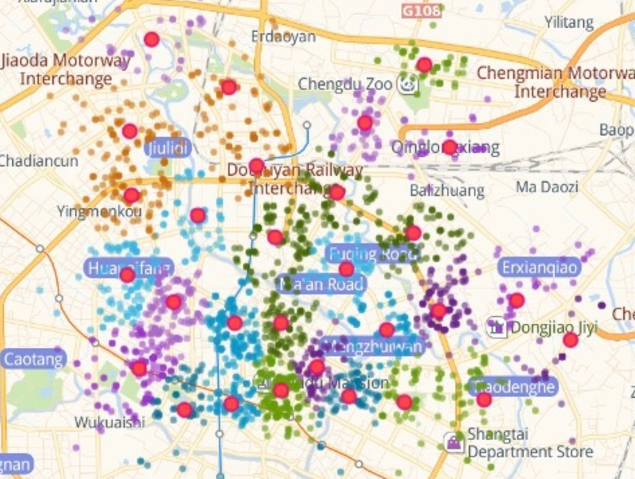
\includegraphics[width=0.5\linewidth]{fig/station_new.pdf}
    \caption{30 selected destination stations.}
    \label{fig:station}
\end{figure}

\color{blue}

\subsubsection{Uncertainty Generation}
We simulate dynamic market environments by introducing stochastic volatility. We model the order arrival process as a Non-Homogeneous Poisson Process (NHPP). Based on the historical demand baseline $\lambda_{base}$, the time-varying intensity $\lambda(t)$ is modeled as:
\begin{equation}
    \lambda(t) = \lambda_{base} \cdot (1 + A \sin(\omega t + \varphi))
\end{equation}
where $A$ controls the \textbf{Uncertainty Scale} and $\omega$ controls the \textbf{Uncertainty Frequency}. Specifically, a higher $A$ simulates more drastic deviations, while a larger $\omega$ introduces more rapid temporal fluctuations in market conditions, creating a more challenging dynamic environment.

\subsubsection{Baselines}
Since most existing approaches tackle the problem in a modular fashion, we categorize the baselines based on the architectural complexity and focus on robustness.

\begin{itemize}
    \item \textbf{Representative Two-Stage Baselines:} These methods represent the standard "pipeline" paradigm, where pricing/dispatching and routing are solved sequentially using established algorithms.
    \begin{itemize}
        \item \textbf{DPEA+SubBus~\cite{ref:DPEA, ref_shared_subway}:} A standard baseline combining a TRPO algorithm for order pricing and bus scheduling with a heuristic insertion algorithm called SubBus for routing.
        \item \textbf{PODP+L2i~\cite{ref:PODP, ref:L2i}:} A hybrid approach that couples predictive dynamic pricing with \textit{L2i}, a learning-based iterative routing solver. This baseline represents methods that rely on demand forecasting and iterative search.
    \end{itemize}
    
    \item \textbf{Advanced Robust \& Composite Baselines:} These are state-of-the-art (SOTA) methods that employ sophisticated mechanisms to enhance specific performance metrics like fairness or robustness.
    \begin{itemize}
        \item \textbf{GRC-ELG~\cite{ref:Lei2023, ref:Yoon2024IJCAI}:} A composite framework integrating Goal-Conditioned RL for strategic dispatching with an Ensemble of Local and Global (ELG) attention mechanism for routing.
        \item \textbf{JDRL-POMO~\cite{ref:Sun2022KDD, ref:KwonPOMO2020}:} A strong baseline for robustness. It combines the JDRL dispatching policy with POMO, a routing solver that uses instance augmentation to enhance routing quality.
    \end{itemize}

    \item \textbf{Internal Ablation:}
    \begin{itemize}
        \item \textbf{SACA (Base Model):} The preliminary version of our framework using a flat MLP actor. It serves as a control group to quantify the specific contribution of the Spatio-Temporal Adaptive mechanism.
    \end{itemize}
\end{itemize}

\subsubsection{Implementation Details}
The algorithm is implemented using PyTorch. The complete set of hyperparameters is summarized in Table~\ref{tab:params}.

\begin{table}[htbp]
\caption{\textcolor{blue}{Simulation Parameters and Hyperparameter Settings}}
\label{tab:params}
\centering
\color{blue}
\begin{tabular}{l|l|c}
\hline
\textbf{Category} & \textbf{Parameter} & \textbf{Value} \\
\hline
\multirow{6}{*}{Simulation Environment} 
 & Number of Destinations ($K$) & 30 \\
 & Number of Buses & 10 \\
 & Bus Capacity Limit ($L$) & 30 \\
 & Bus Speed ($v$) & 30 km/h \\
 & Unit Distance Cost ($\beta_d$) & 0.15 \\
 & Demand Base Rate ($\lambda_{base}$) & 20 \\
\hline
\multirow{7}{*}{SAC Algorithm} 
 & Optimizer & Adam \\
 & Learning Rate ($\alpha_{lr}$) & $3 \times 10^{-4}$ \\
 & Discount Factor ($\gamma$) & 0.99 \\
 & Soft Update ($\tau$) & 0.005 \\
 & Batch Size & 256 \\
 & Replay Buffer Size & $100,000$ \\
 & Hidden Layer Units & 256 \\
\hline
\multirow{3}{*}{Attention Mechanism} 
 & Embedding Dimension & 64 \\
 & Number of Heads & 4 \\
 & Attention Layers & 2 \\
\hline
\end{tabular}
\end{table}

\subsection{Performance Comparison (RQ1)}

\color{blue}
\subsubsection{Performance under Stationary Scenarios}
First, we validate the effectiveness of our proposed framework under a stationary environment using historical dataset without synthetic uncertainty injection. As shown in Table~\ref{tab:rev}, ST-SACA consistently outperforms the representative two-stage baselines significantly accross different settings. ST-SACA achieves the highest profit with a relatively shorter total travel distance compared to baselines. This confirms that our end-to-end joint optimization strategy can effectively filter out low-value, high-cost orders that multi-stage methods fail to identify, thereby optimizing the long-term profitability of the platform.

\begin{table}[htbp]
\caption{\textcolor{blue}{Performance Comparison under Stationary Scenario}}
\label{tab:rev}
\begin{center}
\color{blue}
\setlength{\tabcolsep}{1.7mm}{
\begin{tabular}{c|c|c|c|c|c|c}
\hline
Bus Count & \multicolumn{3}{c|}{10 Buses} & \multicolumn{3}{c}{20 Buses} \\
\hline
Method & Profit & ORR & Length  & Profit & ORR & Length\\
\hline
DPEA+SubBus & 16.63 & 0.08 & 13.75 & 38.97 & 0.18 & 16.89\\
PODP+L2i & 20.03 & 0.13 & 18.16 & 45.12 & 0.24 & 20.45\\
SACA & 23.25 & 0.10 & 12.17 & 53.97 & 0.21 & 15.85\\
\textbf{ST-SACA} & \textbf{38.00} & \textbf{0.18} & \textbf{17.73} & \textbf{73.35} & \textbf{0.28} & \textbf{18.51}\\
\hline
\end{tabular}}
\end{center}
\end{table}

\color{blue}

\subsubsection{Performance under Non-Stationary Scenarios}
To evaluate the robustness of our framework against environmental uncertainty, we conducted experiments with perturbation parameters $A=5$ and $\omega=1$. Table~\ref{tab:rev_uncertainty} summarizes the quantitative results, and Figure~\ref{fig:exper_curve} illustrates the training dynamics across different metrics. ST-SACA not only yields higher profit but also ensures better public service quality and training stability under uncertain conditions.

As shown in Table~\ref{tab:rev_uncertainty}, ST-SACA demonstrates a significant performance advantage over all baselines. Specifically, ST-SACA achieves the highest reward and profit, which demonstrates that by explicitly modeling topological dependencies via the Spatio-Temporal Adaptive Actor, ST-SACA effectively mitigates the impact of random noise, leading to superior decision-making robustness. Besides, ST-SACA strikes the best balance between operational cost and service quality. It achieves the highest ORR while maintaining a moderate cost. This demonstrates that our model is capable of identifying and fulfilling high-value orders—even those requiring complex routing—thereby maximizing the composite Total Reward. In constract, JDRL-POMO's ORR is remarkably low, indicating a conservative strategy that prioritizes cost minimization over service coverage. GRC-ELG achieves a better ORR but incurs the highest operational cost, suggesting an inefficient routing logic when demand density increases.

Through the learning process depicted in Figure~\ref{fig:exper_curve}, we observe that ST-SACA not only attains higher final performance but also exhibits superior training stability compared to baselines. ST-SACA converges to a stable, high-reward policy, which confirms the effectiveness of the entropy-regularized objective in our SAC framework. The ORR curve reveals the another core driver of our performance. While baselines plateau around $0.09-0.16$, ST-SACA continuously learns to expand its service coverage, stabilizing at $\approx 0.18$. This implies that as training progresses, the Spatio-Temporal Actor becomes increasingly proficient at coordinating fleet resources to cover "hotspot" areas dynamically.

\begin{table}[htbp]
\caption{\textcolor{blue}{Performance Comparison under Non-Stationary Scenario}}
\label{tab:rev_uncertainty}
\begin{center}
\color{blue}
\setlength{\tabcolsep}{3.5mm}{
\begin{tabular}{c|c|c|c|c}
\hline
Method & Reward & Profit & Cost & ORR \\
\hline
SACA & 21.70 & 21.33 & 12.11 & 0.09 \\
GRC-ELG & 33.34 & 32.68 & 19.21 & 0.16 \\
JDRL-POMO & 24.86 & 24.50 & \textbf{9.65} & 0.09 \\
\textbf{ST-SACA} & \textbf{38.70} & \textbf{38.00} & 17.73 & \textbf{0.18} \\
\hline
\end{tabular}}
\end{center}
\end{table}

\begin{figure}[htbp]
    \centering
    \captionsetup[subfloat]{font=scriptsize} % 局部缩小该组子图标题字号
    % 第一行：Reward 和 Profit
    \subfloat[Reward]{
        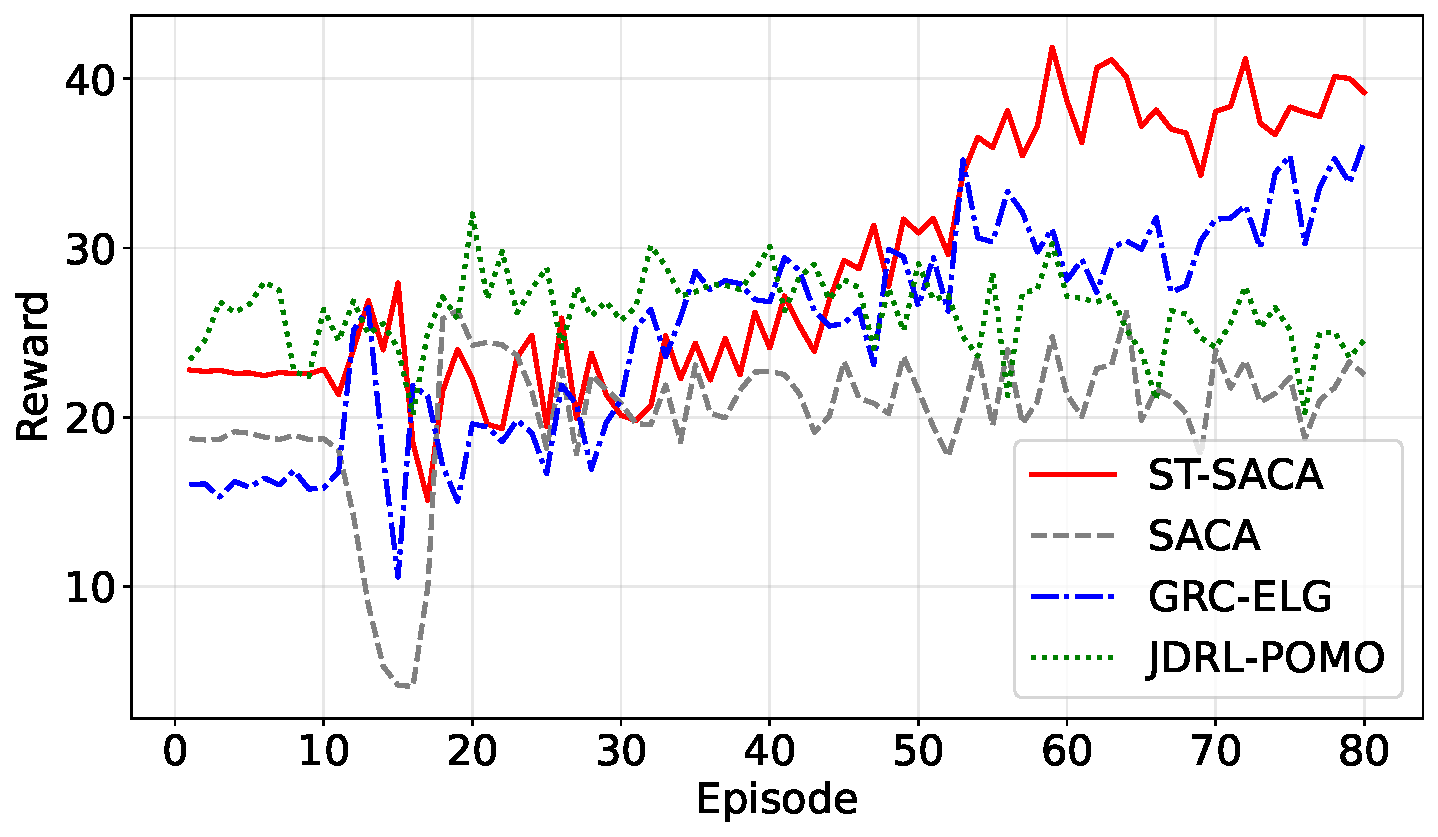
\includegraphics[width=0.47\columnwidth]{fig/comparison_total_reward.pdf}
        \label{fig:curve_reward}
    }
    \hfill
    \subfloat[Profit]{
        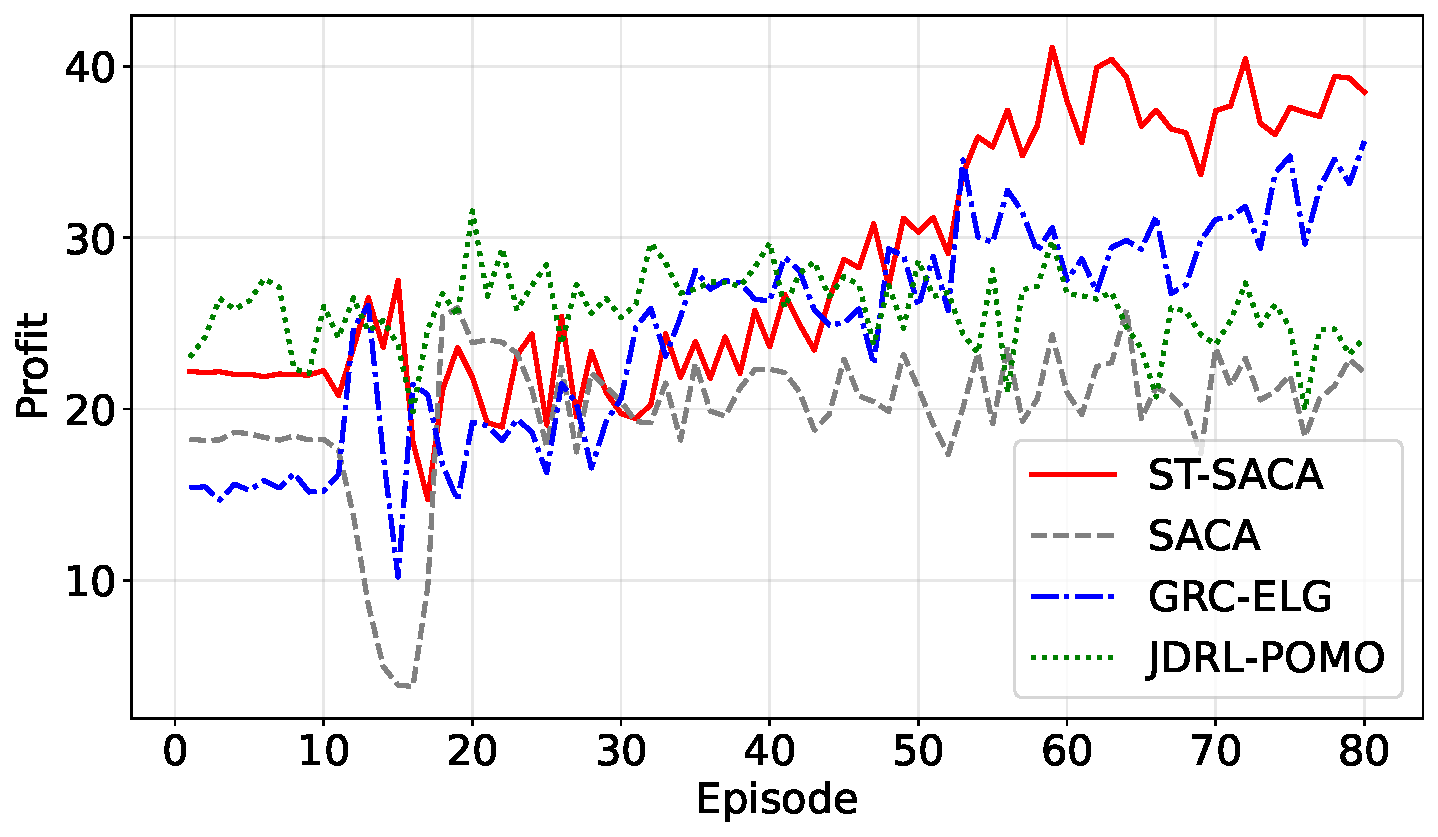
\includegraphics[width=0.47\columnwidth]{fig/comparison_revenue.pdf}
        \label{fig:curve_profit}
    }
    \\ % 换行
    % 第二行：Cost 和 ORR
    \subfloat[Cost]{
        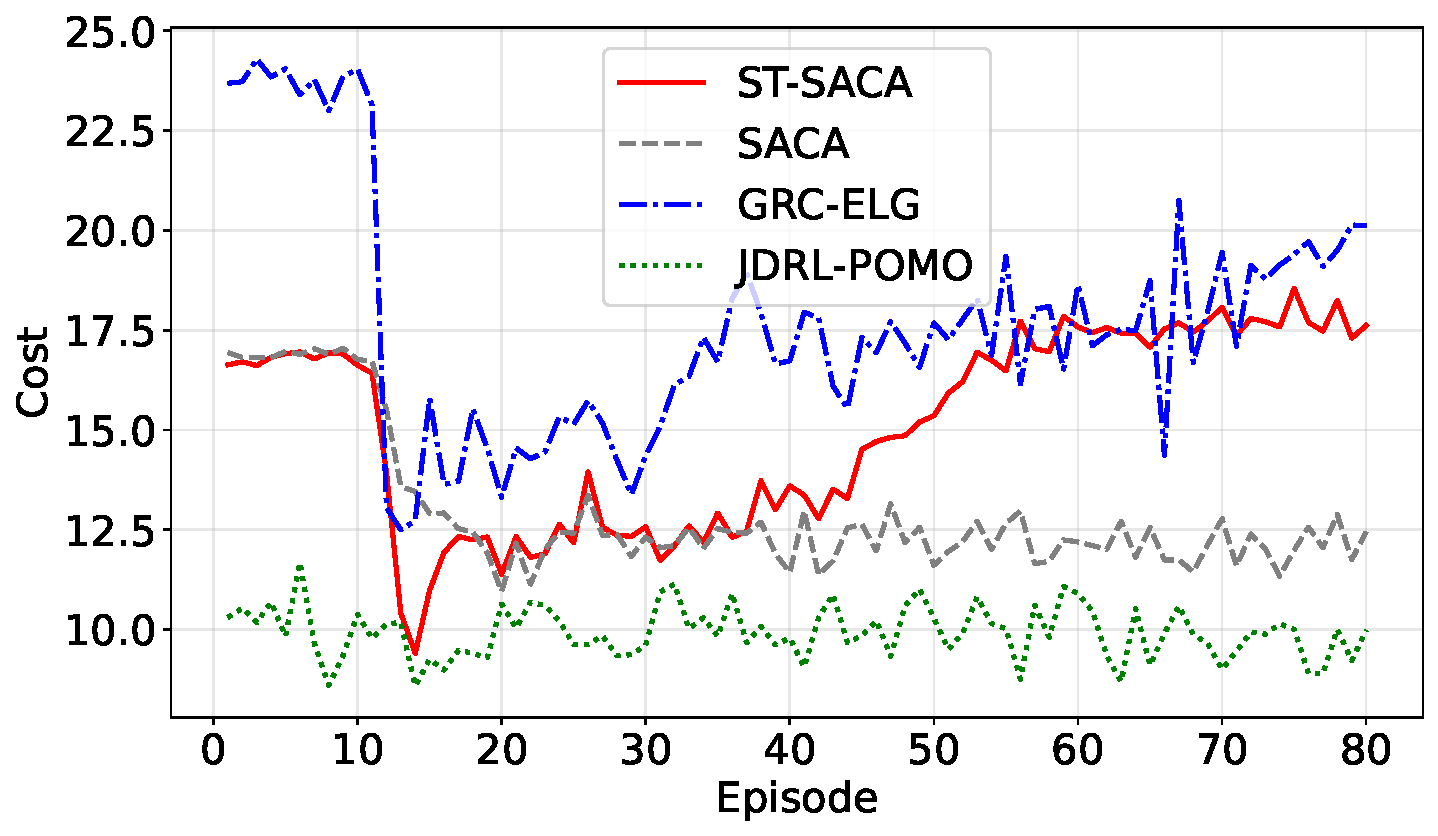
\includegraphics[width=0.47\columnwidth]{fig/comparison_cost.pdf}
        \label{fig:curve_cost}
    }
    \hfill
    \subfloat[ORR]{
        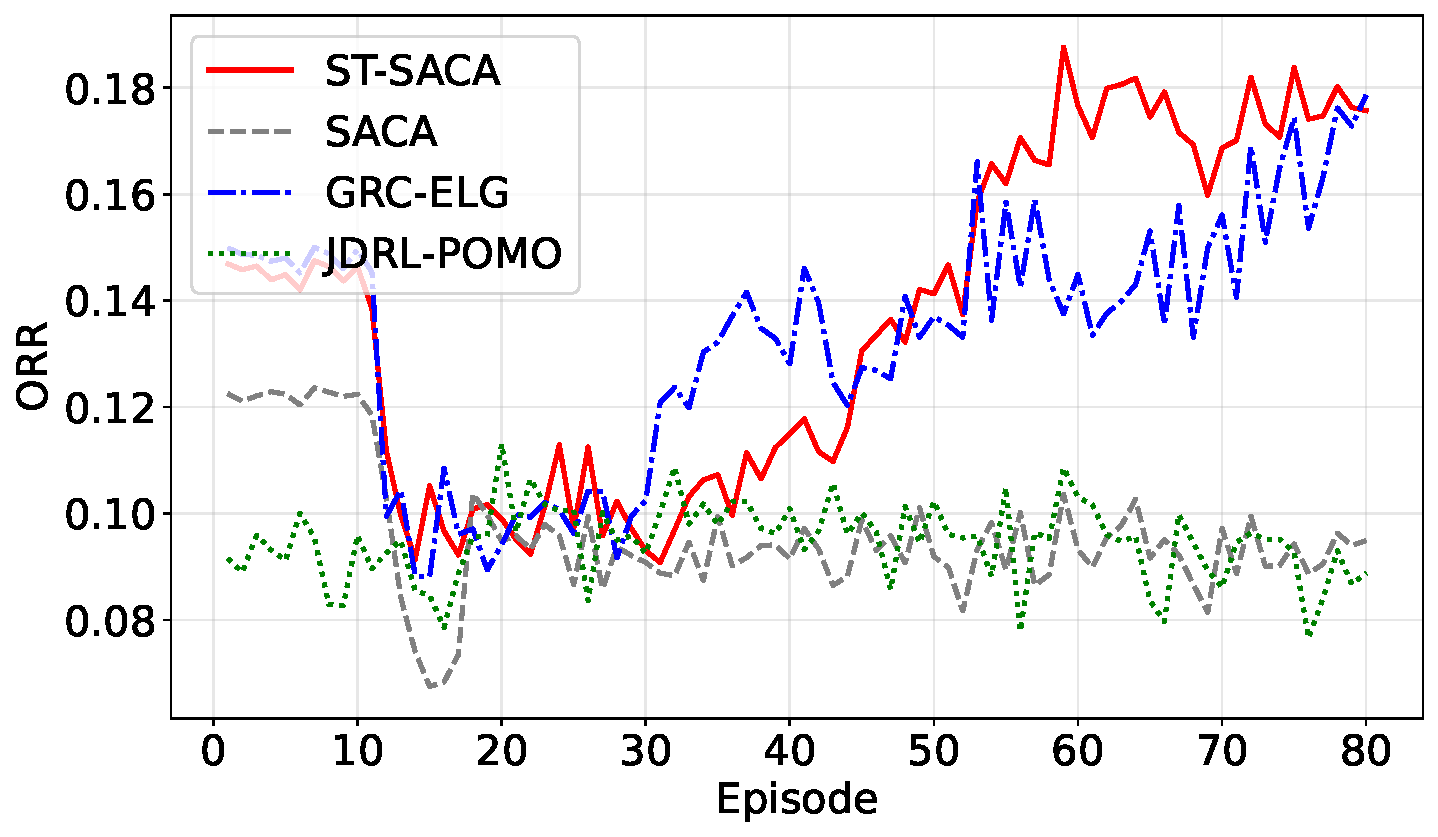
\includegraphics[width=0.47\columnwidth]{fig/comparison_orr.pdf}
        \label{fig:curve_orr}
    }
    \caption{\textcolor{blue}{Training curves of different methods under non-stationary scenarios. The subplots illustrate the evolution of Reward, Profit, Cost, and ORR during the training process. ST-SACA (red solid line) outperforms comparative methods by achieving better convergence values, demonstrating faster convergence and better stability in non-stationary environments.}}
    \label{fig:exper_curve}
\end{figure}

\subsubsection{Impact of Uncertainty Degree (RQ2)}

To further investigate the robustness of ST-SACA, we evaluate the performance of different models under varying uncertainty configurations. By increasing $A$ and $\omega$, the environment exhibits higher variability, presenting a greater challenge for stable decision-making. Table~\ref{tab:uncertainty_full} summarizes the performance gap between ST-SACA and the strongest performing baseline under four distinct uncertainty settings. 

In the scenario with low uncertainty ($A=1, \omega=0.5$), the environment is relatively stable. Here, the performance gap between ST-SACA and the best baseline is marginal (+2.8\%). This observation is consistent with expectations, as baselines can perform adequately when traffic demand is stationary. However, as the environment becomes more volatile, the superiority of ST-SACA becomes increasingly pronounced. The gap further widens to $16.1\%$, which demonstrates that ST-SACA can exploit the structural dependencies in the station network to capture dynamic opportunities that baselines miss. This confirms that our framework is reliable for real-world deployment where extreme demand volatility is inevitable.

% \begin{table}[htbp]
% \caption{Profit under Differnt Uncertainty}
% \label{tab:uncertainty_gap}
% \begin{center}
% \setlength{\tabcolsep}{2mm}{
% \begin{tabular}{c|c|c|c}
% \hline
% Uncertainty Setting $(A, \omega)$ & ST-SACA & Best Baseline & Gap (\%) \\
% \hline
% $A=1,\, \omega=0.5$  & 30.18 & 29.35 & +2.8\%  \\
% $A=1,\, \omega=1$    & 30.23 & 27.27 & +10.9\% \\
% $A=5,\, \omega=1$    & 40.19 & 36.21 & +11.0\% \\
% $A=10,\, \omega=1$   & 38.70 & 33.34 & +16.1\% \\
% \hline
% \end{tabular}}
% \end{center}
% \end{table}

\begin{table}[htbp]
\caption{\textcolor{blue}{Profit Comparison under Different Uncertainty}}
\label{tab:uncertainty_full}
\begin{center}
\color{blue}
\setlength{\tabcolsep}{1.5mm}{
\begin{tabular}{c|c|c|c|c}
\hline
Uncertainty Setting & ST-SACA & SACA & GRC-ELG & JDRL-POMO \\
\hline
$A=1, \omega=0.5$ & \textbf{30.18} & 22.62 & 29.35 & 27.56 \\
$A=1, \omega=1$   & \textbf{30.23} & 23.32 & 26.31 & 27.27 \\
$A=5, \omega=1$   & \textbf{40.19} & 21.70 & 36.21 & 25.53 \\
$A=10, \omega=1$  & \textbf{38.70} & 20.49 & 33.34 & 24.86 \\
\hline
\end{tabular}}
\end{center}
\end{table}

\subsection{Ablation Study (RQ3)}

To verify the contribution of each component within ST-SACA, we compared the full model against three distinct variants. The results, summarized in Table~\ref{tab:ablation}, isolate the impact of the Spatio-Temporal Adaptive Actor, the Attention-Based Routing, and the service-oriented reward design.

\textbf{1) Impact of Spatio-Temporal Adaptive Actor (w/o Spatial Attn.):} 
Replacing the spatio-temporal attention mechanism with a MLP results in a catastrophic performance degradation. The reward drops by 47.1\%, and the ORR is halved, which indicates that without explicit modeling of topological dependencies, the agent collapses into a ``conservative'' strategy by refusing to serve distant orders. This proves that the spatial attention mechanism is essential for encouraging the agent to explore and exploit spatially distributed demand.

\textbf{2) Impact of Learned Routing (w/o Learned Route):} 
Substituting the learned routing module with a greedy nearest-neighbor heuristic yields a significantly lower reward. This performance gap demonstrates that the attention-based routing module serves as a superior solver that generates proper routes for complex batches. This high-efficiency routing capability empowers the ST-SACA framework to accept and fulfill more challenging order combinations.

\textbf{3) Impact of Service Quality Incentive (w/o ORR Reward):} 
Removing the ORR term from the reward function ($\lambda_{orr}=0$) causes the policy to degenerate into a purely profit-seeking agent. Without the explicit incentive to serve passengers, the agent tends to ``cherry-pick'' only the most convenient orders while ignoring the broader demand. This confirms that the composite reward design is critical for aligning the agent's behavior with the platform's dual goals of profitability and public service responsibility.

The full ST-SACA framework achieves the best balance across all metrics. It leverages spatial attention to perceive demand, learned routing to tackle complex routing scenarios, and a composite reward to maintain high service levels, thereby outperforming all ablated variants.

\begin{table}[htbp]
\caption{\textcolor{blue}{Comparison of ST-SACA Variants}}
\label{tab:ablation}
\begin{center}
\color{blue}
\resizebox{\columnwidth}{!}{
\setlength{\tabcolsep}{1.0mm}{
\begin{tabular}{c|ccccc}
\hline
Variant & Reward & Profit & Cost & ORR & Dist.(km) \\
\hline
\textbf{ST-SACA (Full)} & \textbf{38.70} & \textbf{38.00} & 17.73 & \textbf{0.18} & 118.23 \\
w/o Spatial Attn. & 20.49 & 20.12 & 12.03 & 0.09 & 80.22 \\
w/o Learned Route & 26.98 & 26.62 & \textbf{9.71} & 0.09 & \textbf{64.73} \\
w/o ORR Reward & 26.34 & 25.98 & 9.91 & 0.09 & 66.05 \\
\hline
\end{tabular}}}
\end{center}
\end{table}

\subsection{Computational Efficiency (RQ4)}
Real-time response capability is critical for online bus-booking platforms to ensure timely feedback. We evaluate the computational efficiency of ST-SACA by recording the average inference time per time slot under varying scales of the bus fleet. As presented in Table~\ref{tab:e2e_time}, ST-SACA demonstrates exceptional efficiency, maintaining millisecond-level inference speeds. Specifically, as the fleet size expands from 10 to 50 buses, the decision-making latency increases marginally from 4.7 ms to 12.5 ms. This empirical result confirms that our end-to-end framework is highly scalable and well-suited for real-time deployment in latency-sensitive environments.

\begin{table}[htbp]
\caption{\textcolor{blue}{Inference Time per Time Slot (ms) with Varying Fleet Size}}
\label{tab:e2e_time}
\begin{center}
\color{blue}
\setlength{\tabcolsep}{4mm}{
\begin{tabular}{l|ccccc}
\hline
Bus Num & 10 & 20 & 30 & 40 & 50 \\
\hline
ST-SACA & 4.7 & 5.9 & 8.6 & 11.9 & 12.5 \\
\hline
\end{tabular}}
\end{center}
\end{table}

\subsection{Sensitivity Analysis}
We evaluate the sensitivity of the hyper-parameter $\lambda_{orr}$ to analyze its impact on model performance. As illustrated in Figure~\ref{fig:sen}, both average profit and average ORR exhibit a consistent upward trend as $\lambda_{orr}$ increases from 0 to 400. This indicates that properly responding to more orders is synergistic with profit maximization, as serving more passengers generates additional revenue that outweighs the marginal operational costs. However, when $\lambda_{orr}$ exceeds 400, both metrics begin to decline. This suggests that an excessive weight on ORR may lead to accepting inefficient orders, thereby harming overall profitability and fleet efficiency. It is worth noting that in our main comparison experiments, we adopted a conservative setting of $\lambda_{orr}=4$. This choice demonstrates that ST-SACA is capable of outperforming state-of-the-art baselines even without aggressive parameter tuning, while the sensitivity analysis highlights the framework's potential for further performance gains under optimized configurations.

\begin{figure}[htbp]
    \centering
    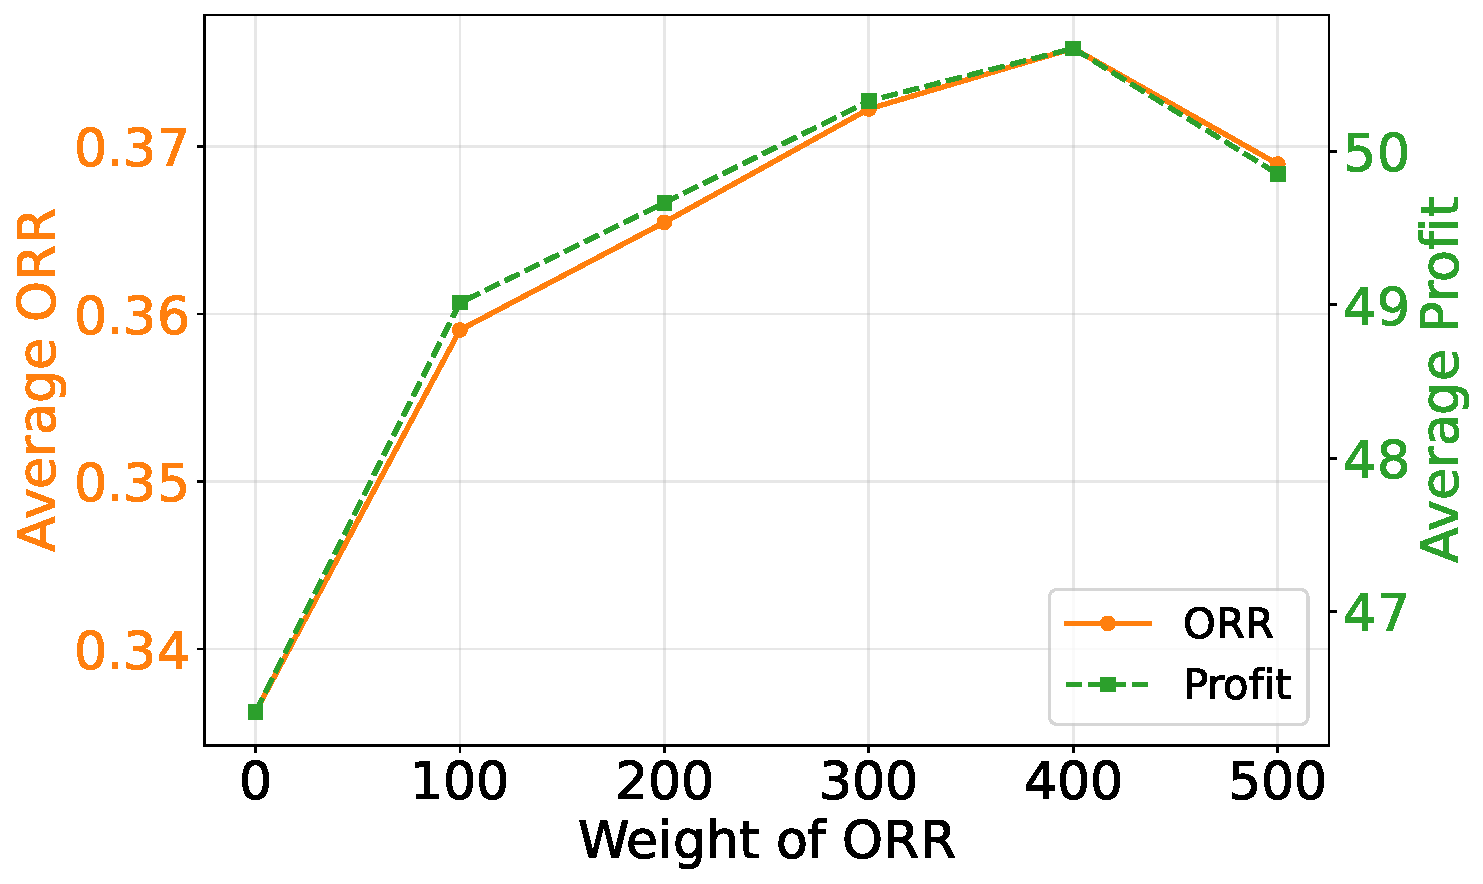
\includegraphics[width=0.6\linewidth]{fig/parameter_sensitivity_orr.pdf}
    \caption{\textcolor{blue}{Performance comparison showing the correlation between Average ORR and Average Profit across different ORR weights.}}
    \label{fig:sen}
\end{figure}

\subsection{Case Study: Pricing Policy}

\begin{figure}[htbp]
    \centering
    % 统一设置子图标题字号为 scriptsize
    \captionsetup[subfloat]{font=scriptsize}
    
    % --- 第一行：三张子图 ---
    \subfloat[Potential demand.]{
        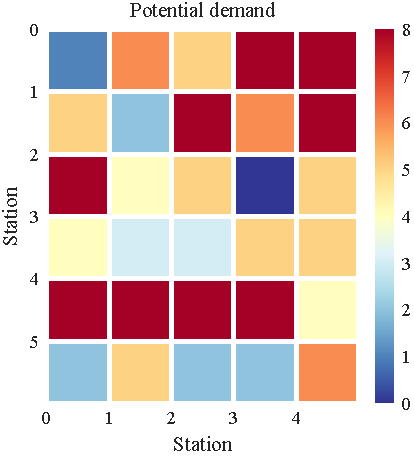
\includegraphics[width=0.3\linewidth, height=2.6cm]{fig/case_study_pricing_demand.pdf}
        \label{fig:pot}
    }
    \hfill
    \subfloat[Pricing of ST-SACA.]{
        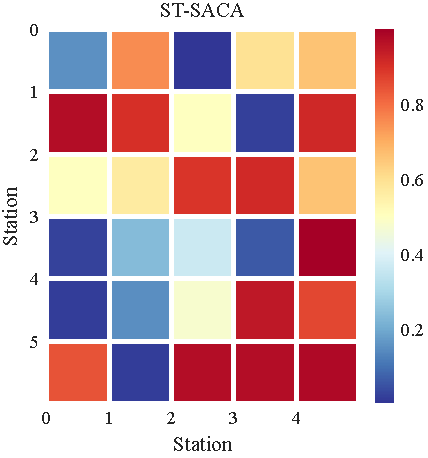
\includegraphics[width=0.3\linewidth, height=2.6cm]{fig/case_study_pricing_st_saca.pdf}
        \label{fig:price_st_saca}
    }
    \hfill
    \subfloat[Pricing of SACA.]{
        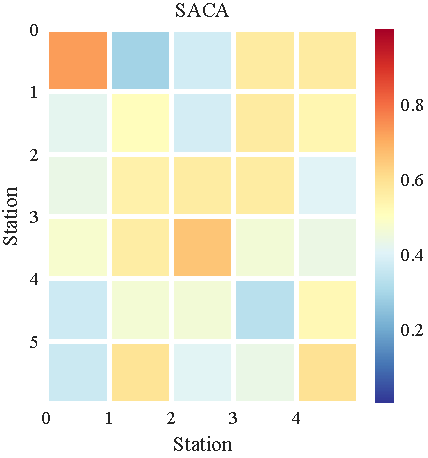
\includegraphics[width=0.3\linewidth, height=2.6cm]{fig/case_study_pricing_saca.pdf}
        \label{fig:price_saca_only}
    }

    \vspace{1mm} % 行间距

    % --- 第二行：两张子图（宽度仍保持 0.31 以确保和上一行图一样大） ---
    % 我们给图片左右各加 0.05\linewidth 的透明边距，标题宽度就变成了 0.31 + 0.1 = 0.41
    \subfloat[Pricing of JDRL-POMO.]{
        \hspace{0.05\linewidth}
        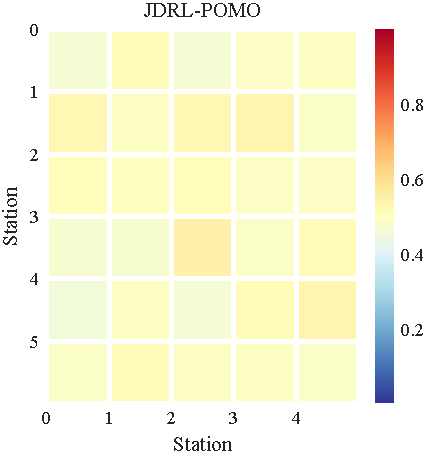
\includegraphics[width=0.3\linewidth, height=2.6cm]{fig/case_study_pricing_jdrl_pomo.pdf}
        \hspace{0.05\linewidth}
        \label{fig:price_jdrl}
    }
    % \hspace{2mm} % 两组子图之间的物理间距
    \subfloat[Pricing of GRC-ELG.]{
        \hspace{0.05\linewidth}
        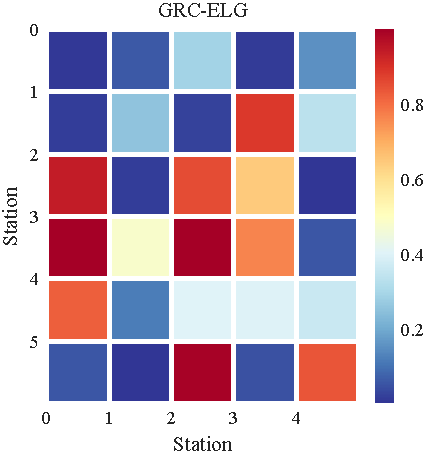
\includegraphics[width=0.3\linewidth, height=2.6cm]{fig/case_study_pricing_grc_elg.pdf}
        \hspace{0.05\linewidth}
        \label{fig:price_grc}
    }

    \caption{\textcolor{blue}{Case study on pricing and demand. ST-SACA  demonstrates an effective pricing strategy compared to baselines.}}
    \label{fig:case_study_all}
\end{figure}

\color{blue}

We conduct a case study to analyze the differences in pricing policies between our proposed ST-SACA and baselines. Figure~\ref{fig:pot} reflects the potential demand of 30 stations. Figure~\ref{fig:price_st_saca} and the baseline figures illustrate the pricing policies. For the station (5,5), which exhibits high potential demand, ST-SACA determines a significantly higher price than all three baselines. This indicates that ST-SACA can effectively explore higher prices for stations with high demand to maximize profit. In contrast, JDRL-POMO tends to set conservatively low prices across the region, while SACA and GRC-ELG fail to capture the peak demand at specific stations. Furthermore, for the peripheral stations in column 4, ST-SACA maintains appropriate high prices to filter out improper orders that might cause detours, whereas the baselines determine lower prices, potentially leading to inefficient routing. Due to the superior spatio-temporal awareness, ST-SACA demonstrates a more effective pricing strategy.



% \section{Discussion}
% \subsection{Scalability}
% The computational complexity of the self-attention mechanism in ST-SACA is $O(N^2)$, where $N$ is the number of stations. In our experiments with $N=30$, the inference time is negligible. However, for city-scale deployments with hundreds of stations, this quadratic complexity could become a bottleneck. Future work could explore \textit{Linear Attention} mechanisms or hierarchical reinforcement learning to handle larger state spaces efficiently.

% \subsection{Real-world Deployment}
% Deploying ST-SACA in a real-world bus-booking system may face the \textit{cold start} problem, where the model lacks sufficient interaction data initially. To address this, we can pre-train the model using a simulator built from historical data (as done in this paper) before online fine-tuning. Additionally, safety constraints should be strictly enforced during the exploration phase to ensure service quality.

\section{Conclusion}
In this paper, we focus on the emerging Bus-Booking service and systematically formulate the Joint Dispatching, Routing, and Pricing (JDRP) problem. To bridge the gap between theoretical simplification and real-world volatility, we explicitly distinguish between two problem variants: the Stationary JDRP (S-JDRP) for stable environments and the Robust JDRP (R-JDRP) under dynamic uncertainty. We propose ST-SACA, a unified end-to-end framework capable of addressing both variants effectively. Distinguished by its Spatio-Temporal Adaptive Actor, ST-SACA integrates geographical coordinates with demand data via a self-attention mechanism. This design captures critical topological dependencies, enabling the agent to learn high-quality strategies while maintaining superior adaptability and robustness. Furthermore, we align the algorithmic optimization with market realities by constructing distance-aware demand-supply functions and a composite reward scheme, balancing profitability with service quality. Extensive experiments on real-world datasets demonstrate that ST-SACA significantly outperforms state-of-the-art baselines in terms of long-term profit and solution quality across both stationary and non-stationary scenarios.

\color{black}

\bibliographystyle{IEEEtran}
\bibliography{ref}

\vspace{-1cm}

\begin{IEEEbiography}[{
\includegraphics[width=1in,height=1.25in,clip,keepaspectratio]{fig/photo/yucengao.jpg}}]{Yucen Gao} is currently an associate professor with the Software College of Northeastern University. He received the B.S. and Ph.D. degree from Shanghai Jiao Tong University, China, in 2020 and 2025. His research interests data engineering and network optimization. He has published more than 20 papers in high-ranked international conferences and journals such as TMC, TON, SIGKDD, SIGIR, ICDE, WWW, etc. 
% More details can be found at https://gaoyucen.github.io.
\end{IEEEbiography}
\vspace{-1cm} % 调整这里，如果觉得太挤就改成 -0.5cm

\begin{IEEEbiography}[{
\includegraphics[width=1in,height=1.25in,clip,keepaspectratio]{fig/photo/pengfeidu.jpeg}}]{Pengfei Du}
is currently a M.S. student at Northeastern University, China (2025--2028), under the supervision of Prof. Xiaochun Yang. He received the B.S. degree (in Information and Computing Science) in 2025. His research interests include data engineering and network optimization.
\end{IEEEbiography}
\vspace{-1cm}

\begin{IEEEbiography}
[{
\includegraphics[width=1in,height=1.25in,clip,keepaspectratio]{fig/photo/Gao.jpg}}]{Xiaofeng Gao}
(Senior Member, IEEE) received the B.S. degree from Nankai University, China, in 2004, the M.S. degree from Tsinghua University, China, in 2006, and the Ph.D. degree from The University of Texas at Dallas, USA, in 2010. She is currently a Full Professor with the School of Computer Science, Shanghai Jiao Tong University, China. Her research interests include data engineering and network optimizations. She has published over 150 peer-reviewed papers in the related area, including well-archived international journals, such as the IEEE TRANSACTIONS ON COMPUTERS, IEEE TRANSACTIONS ON KNOWLEDGE AND DATA ENGINEERING, IEEE TRANSACTIONS ON MOBILE COMPUTING, IEEE TRANSACTIONS ON PARALLEL AND DISTRIBUTED SYSTEMS, and also in well-known conference proceedings, such as SIGKDD, INFOCOM, WWW, ICDE, etc. She has served on the Editorial Board of Discrete Mathematics, Algorithms, and Applications.
\end{IEEEbiography}
\vspace{-1cm}

\begin{IEEEbiography}[{
\includegraphics[width=1in,height=1.25in,clip,keepaspectratio]{fig/photo/binwang.jpg}}]{Bin Wang} received the Ph.D. degree in computer science and technology from Northeastern University, Shenyang, China, in 2008. He is currently a Professor with the School of Computer Science and Engineering, Northeastern University. His research interests include big data management and knowledge engineering, database theory and technology, cloud computing, and data privacy preserving. More details about his research can be found at http://faculty.neu.edu.cn/wangbin.
\end{IEEEbiography}
\vspace{-1cm}

\begin{IEEEbiography}
[{
\includegraphics[width=1in,height=1.25in,clip,keepaspectratio]{fig/photo/xiaochunyang.jpg}}]{Xiaochun Yang} 
(Senior Member, IEEE) received the Ph.D. degree in computer software and theory from Northeastern University, Shenyang, China, in 2001. She is currently a Professor with the Software College, Northeastern University. Her research interests include big data management and knowledge engineering, data quality management, data privacy preserving, and recommender systems. For more information visit the link (http://faculty.neu.edu.cn/yangxiaochun).
\end{IEEEbiography}

\vfill % 防止这一页的内容被强制拉伸到底部

\end{document}
